\documentclass[12pt]{beamer}
\usepackage{../Estilos/BeamerFC}
\usepackage{../Estilos/ColoresLatex}
\usepackage{courier}
\usepackage{listingsutf8}
\usepackage{listings}
\usepackage{xcolor}
\usepackage{textcomp}
\usepackage{color}
\definecolor{deepblue}{rgb}{0,0,0.5}
\definecolor{brown}{rgb}{0.59, 0.29, 0.0}
\definecolor{OliveGreen}{rgb}{0,0.25,0}
% \usepackage{minted}

\DeclareCaptionFont{white}{\color{white}}
\DeclareCaptionFormat{listing}{\colorbox{gray}{\parbox{0.98\textwidth}{#1#2#3}}}
\captionsetup[lstlisting]{format=listing,labelfont=white,textfont=white}
\renewcommand{\lstlistingname}{Código}


\definecolor{Code}{rgb}{0,0,0}
\definecolor{Keywords}{rgb}{255,0,0}
\definecolor{Strings}{rgb}{255,0,255}
\definecolor{Comments}{rgb}{0,0,255}
\definecolor{Numbers}{rgb}{255,128,0}

\makeatletter

\newif\iffirstchar\firstchartrue
\newif\ifstartedbyadigit
\newif\ifprecededbyequalsign

\newcommand\processletter
{%
  \ifnum\lst@mode=\lst@Pmode%
    \iffirstchar%
        \global\startedbyadigitfalse%
      \fi
      \global\firstcharfalse%
    \fi
}

\newcommand\processdigit
{%
  \ifnum\lst@mode=\lst@Pmode%
      \iffirstchar%
        \global\startedbyadigittrue%
      \fi
      \global\firstcharfalse%
  \fi
}

\lst@AddToHook{OutputOther}%
{%
  \lst@IfLastOtherOneOf{=}
    {\global\precededbyequalsigntrue}
    {}%
}

\lst@AddToHook{Output}%
{%
  \ifprecededbyequalsign%
      \ifstartedbyadigit%
        \def\lst@thestyle{\color{orange}}%
      \fi
    \fi
  \global\firstchartrue%
  \global\startedbyadigitfalse%
  \global\precededbyequalsignfalse%
}

\lstset{ 
language=Python,                % choose the language of the code
basicstyle=\footnotesize\ttfamily,       % the size of the fonts that are used for the code
numbers=left,                   % where to put the line-numbers
numberstyle=\scriptsize,      % the size of the fonts that are used for the line-numbers
stepnumber=1,                   % the step between two line-numbers. If it is 1 each line will be numbered
numbersep=5pt,                  % how far the line-numbers are from the code
backgroundcolor=\color{white},  % choose the background color. You must add \usepackage{color}
showspaces=false,               % show spaces adding particular underscores
showstringspaces=false,         % underline spaces within strings
showtabs=false,                 % show tabs within strings adding particular underscores
frame=single,   		% adds a frame around the code
tabsize=2,  		% sets default tabsize to 2 spaces
captionpos=t,   		% sets the caption-position to bottom
breaklines=true,    	% sets automatic line breaking
breakatwhitespace=false,    % sets if automatic breaks should only happen at whitespace
escapeinside={| |},  % if you want to add a comment within your code
stringstyle =\color{OliveGreen},
otherkeywords={as, np.array, np.concatenate, np.linspace, linspace, interpolate.interp1d, kind, plt.plot, .copy, np.arange, np.cos, np.pi, lw, ls, label, splrep, splev, plt.legend, loc, plt.title, plt.ylim, plt.show, sign, math.ceil, math.log, np.sqrt, np.exp, np.zeros, plt.xlabel, plt.ylabel, plt.xlim, np.identity, random, np.dot, np.outer, np.diagonal },             % Add keywords here
keywordstyle = \color{blue},
commentstyle = \color{darkcerulean},
identifierstyle = \color{black},
literate=%
         {á}{{\'a}}1
         {é}{{\'e}}1
         {í}{{\'i}}1
         {ó}{{\'o}}1
         {ú}{{\'u}}1
%
%keywordstyle=\ttb\color{deepblue}
%fancyvrb = true,
}

\lstdefinestyle{FormattedNumber}{%
    literate={0}{{\textcolor{red}{0}}}{1}%
             {1}{{\textcolor{red}{1}}}{1}%
             {2}{{\textcolor{red}{2}}}{1}%
             {3}{{\textcolor{red}{3}}}{1}%
             {4}{{\textcolor{red}{4}}}{1}%
             {5}{{\textcolor{red}{5}}}{1}%
             {6}{{\textcolor{red}{6}}}{1}%
             {7}{{\textcolor{red}{7}}}{1}%
             {8}{{\textcolor{red}{8}}}{1}%
             {9}{{\textcolor{red}{9}}}{1}%
             {.0}{{\textcolor{red}{.0}}}{2}% Following is to ensure that only periods
             {.1}{{\textcolor{red}{.1}}}{2}% followed by a digit are changed.
             {.2}{{\textcolor{red}{.2}}}{2}%
             {.3}{{\textcolor{red}{.3}}}{2}%
             {.4}{{\textcolor{red}{.4}}}{2}%
             {.5}{{\textcolor{red}{.5}}}{2}%
             {.6}{{\textcolor{red}{.6}}}{2}%
             {.7}{{\textcolor{red}{.7}}}{2}%
             {.8}{{\textcolor{red}{.8}}}{2}%
             {.9}{{\textcolor{red}{.9}}}{2}%
             {\ }{{ }}{1}% handle the space
         ,%
          %mathescape=true
          escapeinside={__}
          }



\usetheme{Antibes}
\usecolortheme{seagull}
%\useoutertheme{default}
\setbeamercovered{invisible}
% or whatever (possibly just delete it)
\setbeamertemplate{section in toc}[sections numbered]
\setbeamertemplate{subsection in toc}[subsections numbered]
\setbeamertemplate{subsection in toc}{\leavevmode\leftskip=3.2em\rlap{\hskip-2em\inserttocsectionnumber.\inserttocsubsectionnumber}\inserttocsubsection\par}
% \setbeamercolor{section in toc}{fg=blue}
% \setbeamercolor{subsection in toc}{fg=blue}
% \setbeamercolor{frametitle}{fg=blue}
\setbeamertemplate{caption}[numbered]

\setbeamertemplate{footline}
\beamertemplatenavigationsymbolsempty
\setbeamertemplate{headline}{}


\makeatletter
\setbeamercolor{section in foot}{bg=gray!30, fg=black!90!orange}
\setbeamercolor{subsection in foot}{bg=blue!30}
\setbeamercolor{date in foot}{bg=black}
\setbeamertemplate{footline}
{
  \leavevmode%
  \hbox{%
  \begin{beamercolorbox}[wd=.333333\paperwidth,ht=2.25ex,dp=1ex,center]{section in foot}%
    \usebeamerfont{section in foot} \insertsection
  \end{beamercolorbox}%
  \begin{beamercolorbox}[wd=.333333\paperwidth,ht=2.25ex,dp=1ex,center]{subsection in foot}%
    \usebeamerfont{subsection in foot}  \insertsubsection
  \end{beamercolorbox}%
  \begin{beamercolorbox}[wd=.333333\paperwidth,ht=2.25ex,dp=1ex,right]{date in head/foot}%
    \usebeamerfont{date in head/foot} \insertshortdate{} \hspace*{2em}
    \insertframenumber{} / \inserttotalframenumber \hspace*{2ex} 
  \end{beamercolorbox}}%
  \vskip0pt%
}
\makeatother

\makeatletter
\patchcmd{\beamer@sectionintoc}{\vskip1.5em}{\vskip0.8em}{}{}
\makeatother

%\newlength{\depthofsumsign}
%\setlength{\depthofsumsign}{\depthof{$\sum$}}
% \newcommand{\nsum}[1][1.4]{% only for \displaystyle
%     \mathop{%
%         \raisebox
%             {-#1\depthofsumsign+1\depthofsumsign}
%             {\scalebox
%                 {#1}
%                 {$\displaystyle\sum$}%
%             }
%     }
% }
\def\scaleint#1{\vcenter{\hbox{\scaleto[3ex]{\displaystyle\int}{#1}}}}
\def\scaleoint#1{\vcenter{\hbox{\scaleto[3ex]{\displaystyle\oint}{#1}}}}
\def\bs{\mkern-12mu}

\usetikzlibrary{shapes}
\normalfont
\usepackage{ccfonts}% http://ctan.org/pkg/{ccfonts}
\usepackage[T1]{fontenc}% http://ctan.or/pkg/fontenc
\renewcommand{\rmdefault}{cmr}% cmr = Computer Modern Roman
\linespread{1.3}

\title{Tema 5 - Métodos de Monte Carlo}
\subtitle{Curso de Física Computacional}
\author{M. en C. Gustavo Contreras Mayén}

% \setbeamercolor*{block body}{fg=white,bg=black!10}

\begin{document}
\maketitle
\fontsize{14}{14}\selectfont
\spanishdecimal{.}
\newcommand{\localtextbulletone}{\textcolor{gray}{\raisebox{.45ex}{\rule{.6ex}{.6ex}}}}

\section*{Contenido}
\frame{\tableofcontents[currentsection, hideallsubsections]}

\section{El azar}
\frame{\tableofcontents[currentsection, hideothersubsections]}
\subsection{Introducción}

\begin{frame}
\frametitle{Pregunta inicial}
\begin{center}
\textbf{\textcolor{ao}{¿Qué es el azar?}}
\end{center}
\pause
Una pregunta bastante simple de hacer, pero responderla es difícil.
\end{frame}
\begin{frame}[fragile]
\frametitle{Pregunta similar}
Es algo similar al comentario de San Agustín de Hipona sobre el tiempo{\footnote{Confessiones lib xi, cap xiv, sec 17, circa 400 AD.}}:
\\
\pause
\begin{quote}
¿Qué es, entonces, el tiempo? Si nadie me pregunta, lo sé; si quiero explicarle al que pregunta, no sé.
\end{quote}
\pause
Todos pensamos que sabemos qué es el azar cuando lo vemos, pero no podemos explicarlo.
\end{frame} 
\begin{frame}
\frametitle{Nos enfocaremos a las secuencias aleatorias}
Afortunadamente para nosotros, realmente no necesitamos saber qué es la aleatoriedad, lo que realmente nos preocupa aquí es la idea de una \textbf{\textcolor{armygreen}{secuencia aleatoria}}.
\end{frame}
\begin{frame}
\frametitle{Definiendo el concepto}
Definiremos una \textbf{secuencia aleatoria} como una secuencia de números, $n$, dentro de un rango acotado, donde no es posible predecir $n_{k+1}$ de cualquier combinación de valores precedentes $n_{i}, \, i = 0, 1, \ldots, k$.
\end{frame}
\begin{frame}
\frametitle{Definiendo el concepto}
Vemos una secuencia aleatoria como un generador que da un valor cuando se le pregunta sin que podamos predecir ese valor en función de cualquiera de los valores anteriores.
\end{frame}
\begin{frame}
\frametitle{Definiendo el concepto}
Nuestra definición no ha especificado una \textbf{\textcolor{red}{distribución principal}}.
\\
\bigskip
\pause
Los procesos aleatorios a menudo se consideran extracciones de una distribución de probabilidad principal.
\end{frame}
\begin{frame}
\frametitle{Tipo de distribución}
De modo que, aunque no podemos predecir $n_{k}$, \pause podemos aproximarnos a la distribución principal extrayendo repetidamente del proceso aleatorio y construyendo un histograma.
\end{frame}
\begin{frame}
\frametitle{Tipo de distribución}
Aquí \enquote{extraer} significa pedirle al generador otro valor. 
\\
\bigskip
\pause
Para nuestros propósitos, a menos que se indique lo contrario, asumimos que la distribución principal es \textbf{\textcolor{beaver!80!black}{uniforme}}.
\end{frame}
\begin{frame}
\frametitle{Distribución uniforme}
Esto significa que cualquier valor en el rango permitido de valores que podría devolver el generador es tan probable como cualquier otro valor.
\end{frame}
\begin{frame}
\frametitle{Diferentes Distribuciones}
A continuación se muestran histogramas creados por muestreo repetido de un proceso aleatorio con una distribución principal específica.
\end{frame}
\begin{frame}
\frametitle{Distribución binomial}
\begin{figure}
    \centering
    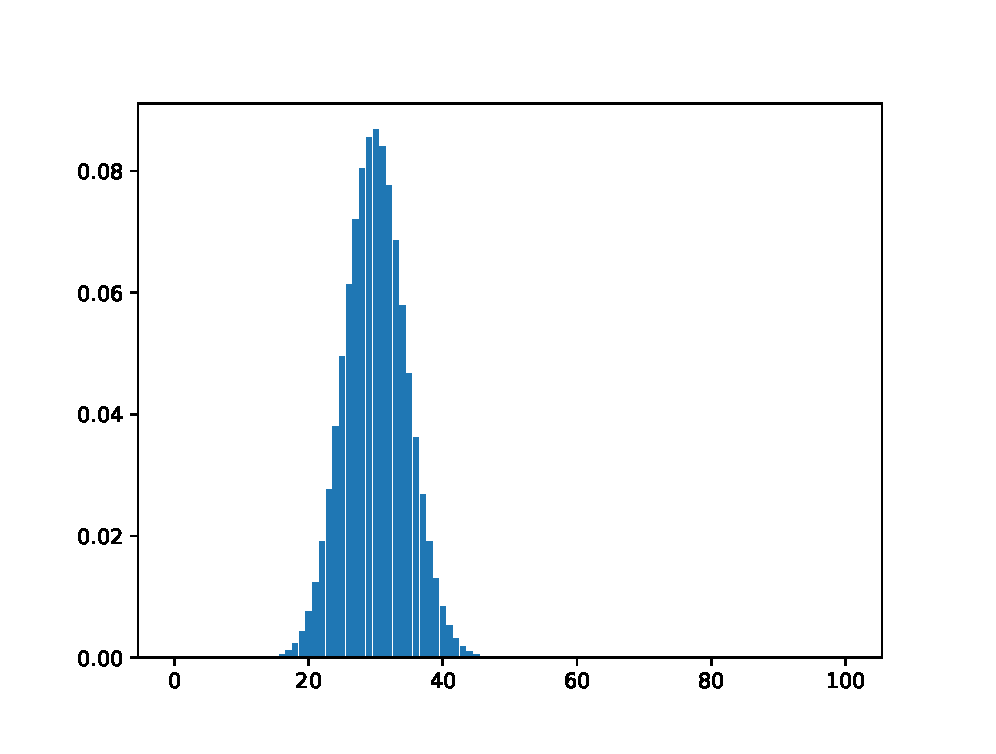
\includegraphics[scale=0.55]{Imagenes/plot_distribucion_01_binomial.eps}
\end{figure}
\end{frame}
\begin{frame}
\frametitle{Distribución uniforme}
\begin{figure}
    \centering
    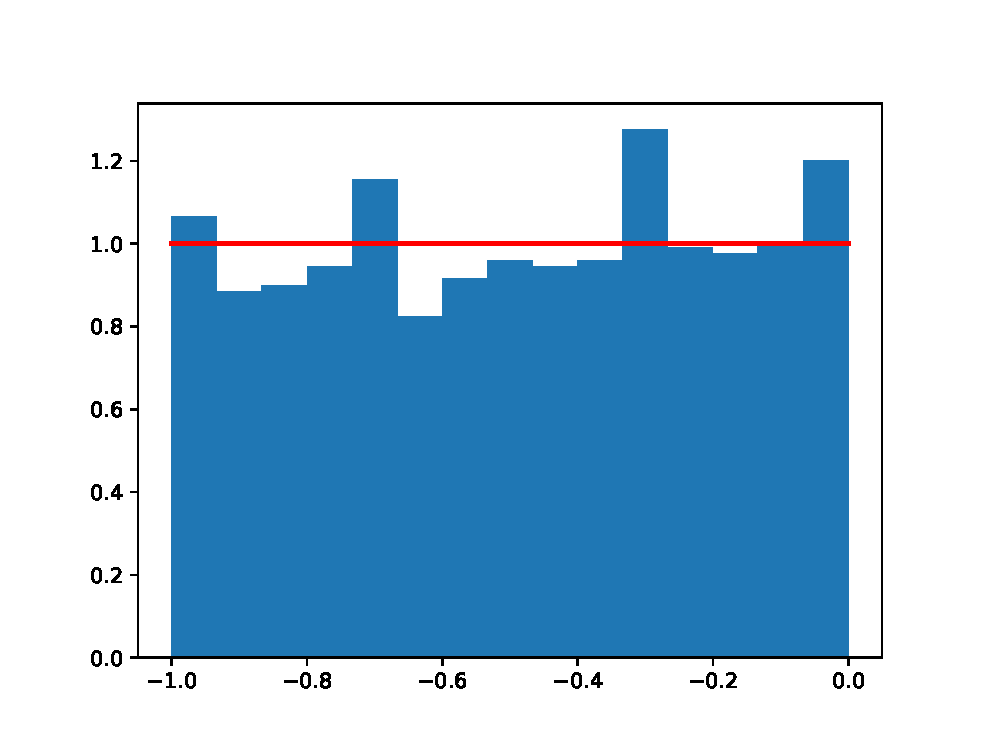
\includegraphics[scale=0.55]{Imagenes/plot_distribucion_02_uniforme.eps}
\end{figure}
\end{frame}
\begin{frame}
\frametitle{Distribución Gaussiana}
\begin{figure}
    \centering
    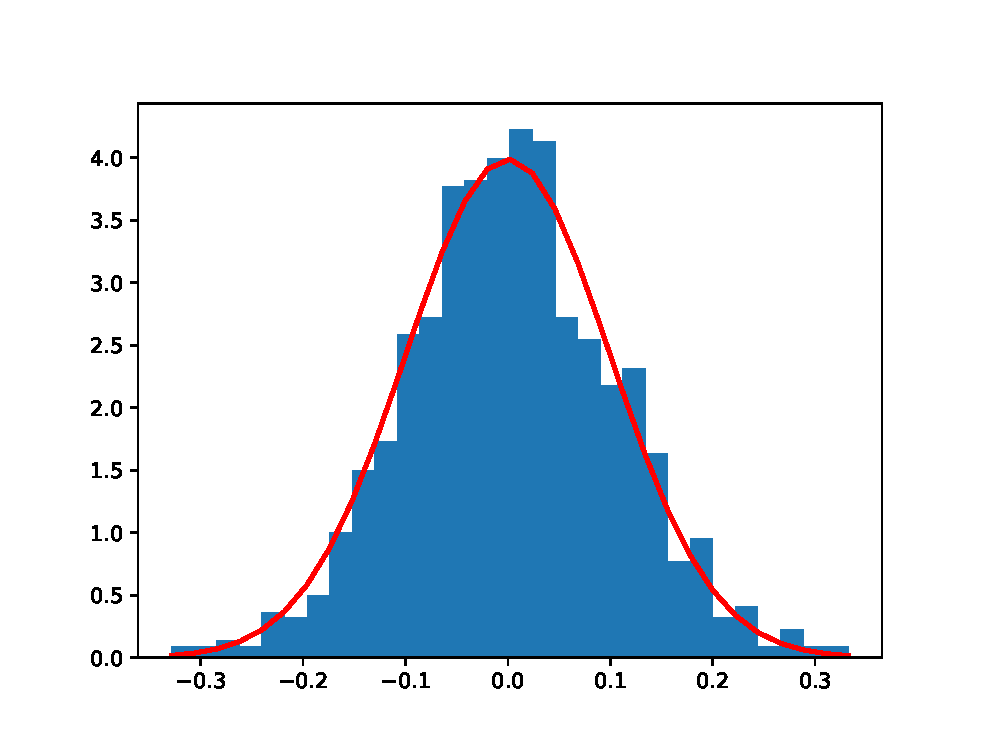
\includegraphics[scale=0.55]{Imagenes/plot_distribucion_03_gaussiana.eps}
\end{figure}
\end{frame}
\begin{frame}
\frametitle{De los datos obtenidos}
Los datos utilizados se basan en la salida de buenos \textocolor{red}{generadores} de números pseudoaleatorios conocidos, \pause pero por el momento los tomaremos como ejemplos de procesos aleatorios reales y las secuencias que generan.
\end{frame}
\begin{frame}
\frametitle{Secuencias aleatorias}
Dejando de lado la filosofía, supondremos que las secuencias aleatorias realmente existen y se encuentran en el mundo físico.
\end{frame}
\begin{frame}
\frametitle{Ejemplos de secuncias aleatorias}
Por ejemplo, tomamos los siguientes como ejemplos de procesos aleatorios a partir de los cuales se podría generar una secuencia aleatoria:
\pause
\setbeamercolor{item projected}{bg=amethyst,fg=white}
\setbeamertemplate{enumerate items}{%
\usebeamercolor[bg]{item projected}%
\raisebox{1.5pt}{\colorbox{bg}{\color{fg}\footnotesize\insertenumlabel}}%
}
\begin{enumerate}[<+->]
\item Lanzar una moneda justa.
\item Tirar un dado justo.
\item La desintegración de los elementos radiactivos.
\item El patrón de estática en un viejo televisor CRT sintonizado en un canal vacío.
\end{enumerate}
\end{frame}
\begin{frame}
\frametitle{Aclaraciones}
En cierto sentido, solo el número tres anterior es verdaderamente aleatorio en el sentido de que se rige por la mecánica cuántica.
\\
\bigskip
\pause
El número cuatro también lo es, hasta cierto punto.
\end{frame}

\section{Métodos de Monte Carlo}
\frame{\tableofcontents[currentsection, hideothersubsections]}
\subsection{Definición}

\begin{frame}
\frametitle{Definición}
El \textocolor{brickred}{método de Monte Carlo} es un conjunto de métodos numéricos que permiten resolver problemas físicos y matemáticos mediante la simulación de variables aleatorias.
\end{frame}
\begin{frame}
\frametitle{Definición}
Los métodos de Monte Carlo fueron nombrados de esta manera por su clara analogía con los juegos de ruleta de los casinos, el más célebre de los cuales es el de Montecarlo, casino cuya construcción fue propuesta en 1856 por el príncipe Carlos III de Mónaco, siendo inaugurado en 1861.
\end{frame}
\begin{frame}
\frametitle{Relevancia del método}
La importancia actual de los métodos Monte Carlo \textbf{se basa en} \pause la existencia de problemas que tienen difícil solución por métodos exclusivamente analíticos o numéricos, \pause pero que dependen de factores aleatorios o se pueden asociar a un modelo probabilístico artificial (resolución de integrales de muchas variables, minimización de funciones, etc.)
\end{frame}
\begin{frame}
\frametitle{Relevancia del método}
Gracias al continuo diseño de procesadores y de computadoras, los cálculos con Monte Carlo que en otro tiempo hubieran sido inconcebibles, hoy en día se presentan como asequibles para la resolución de ciertos problemas.
\end{frame}
\begin{frame}
 \frametitle{Proporción del error}
En estos métodos el error $\simeq \frac{1}{\sqrt{N}}$, donde $N$ es el número de pruebas, por tanto, ganar una cifra decimal en la precisión implica aumentar $N$ en $100$ veces.
\end{frame}
\begin{frame}
\frametitle{Fundamento del método}
La base del método es la generación de números aleatorios de los que nos serviremos para calcular probabilidades.
\\
\bigskip
\pause
Conseguir un buen generador de estos números así como un conjunto estadístico adecuado sobre el que trabajar son las primeras dificultades con las que nos encontraremos a la hora de utilizar este método.
\end{frame}

\subsection{Secuencia aleatoria}

\begin{frame}
\frametitle{Secuencia aleatoria}
Se define una \textocolor{darkmagenta}{secuencia aleatoria} de números $r_{1}, r_{2}, \ldots$ si no existe una correlación entre ellos.
\\
\bigskip
\pause
Aunque sean aleatorios, no implica que todos los números en la secuencia tengan la misma probabilidad de ocurrir.
\end{frame}
\begin{frame}
\frametitle{Secuencia aleatoria}
Si todos los números en la secuencia tienen la misma probabilidad de ocurrir, se dice que la \textocolor{burgundy}{secuencia es uniforme} y los \textocolor{red}{números son aleatorios}.
\\
\bigskip
\pause 
Por ejemplo: $1, 2, 3, 4, \ldots$ es uniforme pero probablemente no es aleatoria.
\end{frame}
\begin{frame}
\frametitle{Secuencia aleatoria}
También es posible tener una secuencia de números que de alguna forma son aleatorios, pero tienen correlación dentro de un intervalo pequeño:
\pause
\begin{align*}
r_{1},  \: (1 - r_{1} ), \: r_{2}, \: (1 - r_{2} ), \: r_{3}, \: (1 - r_{3} ), \: \ldots
\end{align*}
Las computadoras por naturaleza, son determinísticas y \textocolor{darkgreen}{no pueden crear} una secuencia de números aleatorios.
\end{frame}
\begin{frame}
\frametitle{Secuencia aleatoria}
Las computadoras pueden crear secuencias que contengan \textocolor{lava}{correlaciones} y por tanto no ser totalmente aleatorias; si conocemos $r_{m}$ y su elemento precedente, es posible estimar $r_{m+1}$.
\\
\bigskip
\pause
Por ésta razón, se dice que las computadoras son generadores de \textocolor{cordovan}{números pseudoaleatorios}.
\end{frame}
\begin{frame}
\frametitle{Secuencia aleatoria}
Matemáticamente, la probabilidad de que un número ocurra, está descrita por una función de distribución $P(r)$, \pause donde $P (r) \dd{r}$, es la probabilidad de encontrar $r$ en un intervalo $[r, r + \dd{r}]$.
\\
\bigskip
\pause
Una distribución uniforme significa que $P (r) = \mbox{ constante}$.
\end{frame}
\begin{frame}
\frametitle{Generador de número aleatorios}
El \textocolor{cadet}{generador estándar} de números aleatorios en las computadoras, genera distribuciones uniformes entre $0$ y $1$.
\\
\bigskip
\pause 
El generador estándar de números aleatorios, proporciona números en éste intervalo, y cada uno de ellos tiene la misma probabilidad de ocurrir, y además es independiente del número anterior.
\end{frame}

\subsection{Generación de números aleatorios}

\begin{frame}
\frametitle{Generación de números aleatorios}
El método de \textocolor{darkraspberry}{congruencia lineal} es la manera más común que se utiliza para generar una secuencia de números pseudoaleatorios $0 \leq r_{i} \leq M - 1$ en el intervalo $[0, M - 1]$.
\end{frame}
\begin{frame}
\frametitle{Generación de números aleatorios}
Podemos multiplicar el número aleatorio previo $r_{i-1}$ por una constante $a$, \pause sumar otra constante $c$, \pause operar con el módulo $M$, manteniendo sólo la parte fraccional del resultado como el siguiente número aleatorio $r_{i+1}$:
\pause
\begin{align*}
r_{i+1} = (a \; r_{i} + c) \text{ mod } M
\end{align*}
\end{frame}
\begin{frame}
\frametitle{De la semilla}
\begin{align*}
r_{i+1} = (a \; r_{i} + c) \text{ mod } M
\end{align*}
El valor de $r_{1}$ se le llama \textocolor{denim}{semilla} (\textbf{seed}, en inglés) y lo proporciona normalmente el usuario.
\end{frame}
\begin{frame}
\frametitle{Ejemplo}
Veamos la secuencia que se genera si $c = 1$, $a = 4$, $M = 9$, y la semilla es $r_{1} = 3$:
\pause
\begin{align*}
r_{i+1} = (a \; r_{i} + c) \mbox{ mod } M 
\end{align*}
\begin{eqnarray*}
\begin{aligned}
r_{1} &= 3 \\ \pause
r_{2} &= (4 \times 3  + 1) \mbox{ mod } 9 = 13 \mbox{ mod } 9 = 4 \\ \pause
r_{3} &= (4 \times 4  + 1) \mbox{ mod } 9 = 17 \mbox{ mod } 9 = 8 \\ \pause
r_{4} &= (4 \times 8  + 1) \mbox{ mod } 9 = 33 \mbox{ mod } 9 = 6 \\ \pause
r_{5 - 10} &= 7, 2, 0, 1, 5, 3
\end{aligned}
\end{eqnarray*}
\end{frame}
\begin{frame}
\frametitle{Secuencia obtenida}
Hemos obtenido una secuencia de longitud $M = 9$, antes de que la secuencia se repitiera.
\\
\bigskip
\pause
Si queremos números en el rango $[0, 1]$, basta dividir los números $r$ por $M = 9$:
\pause
\begin{align*}
0.333, 0.222, 0.444, 0.000, 0.889, \\
0.111, 0.667, 0.555, 0.778, 0.333
\end{align*}
\end{frame}
\begin{frame}
\frametitle{Factor de escala}
Aún sigue siendo una secuencia de longitud $9$ pero ya no es una secuencia de enteros.
\\
\bigskip
\pause
Si queremos que los números aleatorios estén en el rango $[A, B]$, se requiere aplicar el factor de escala:
\pause
\begin{align*}
x_{i} = A + (B - A) \; r_{i} \hspace{1cm} 0 \leq r_{1} \leq 1 \rightarrow A \leq x_{i} \leq B
\end{align*}
\end{frame}
\begin{frame}
\frametitle{Sugerencia}
Antes de utilizar un generador de números aleatorios en nuestros programas, debemos de revisar que el rango que produce, tiene apariencia de aleatorios.
\end{frame}
\begin{frame}
\frametitle{Sugerencia}
Propiamente \textocolor{amethyst}{no es un prueba matemática}, \pause pero al graficar la distribución de números aleatorios, podemos reconocer ciertos patrones, con lo que nos diría si tenemos o no, números aleatorios.
\end{frame}
\begin{frame}[plain, allowframebreaks, fragile]
\frametitle{Código para los números aleatorios}
\begin{lstlisting}[caption=Código para generar un conjunto de números aleatorios]
x = []

a, semilla, c, m, n = 128, 10, 0, 509, 500
for i in range (1, n):
   nuevasemilla = (a * semilla + c) % m
   semilla = nuevasemilla
   x.append(nuevasemilla)

y = []

a, semilla, c, m, n = 269, 10, 0, 2048, 500

for i in range (1, n):
   nuevasemilla = (a * semilla + c) % m
   semilla = nuevasemilla
   y.append(nuevasemilla)

# Hay que graficar cada lista
\end{lstlisting}
\end{frame}
\begin{frame}[fragile]
\frametitle{Distribución de números aleatorios (1/2)}
\begin{figure}
  \centering
  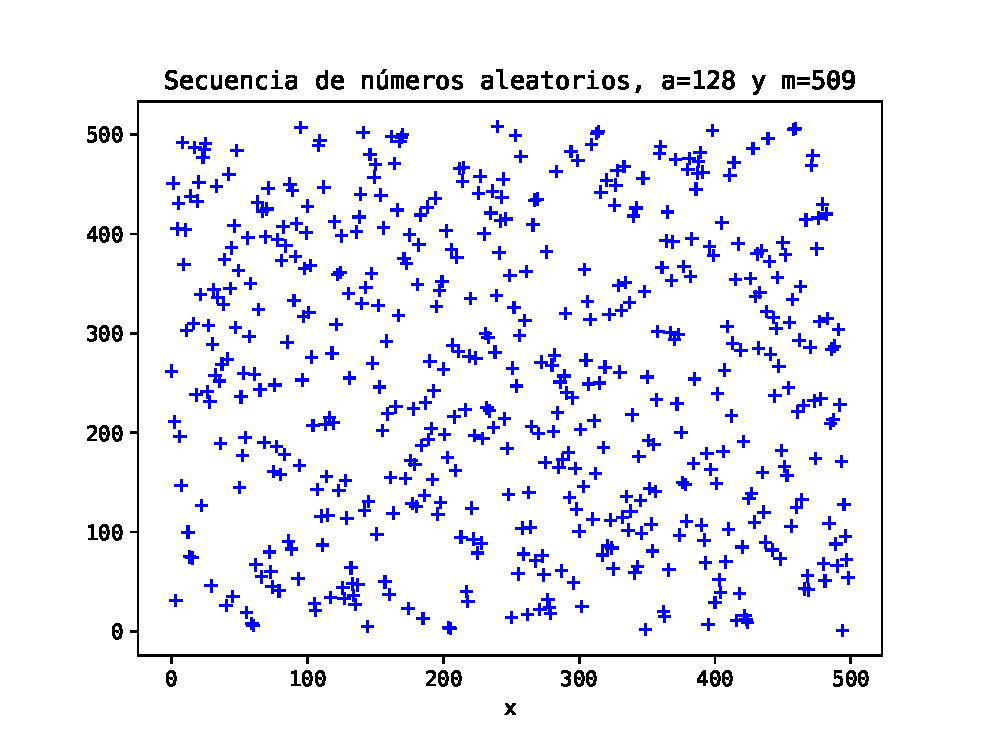
\includegraphics[scale=0.6]{Imagenes/Secuencia_aleatoria_01.eps}
\end{figure}
\end{frame}
\begin{frame}[fragile]
\frametitle{Distribución de números aleatorios (1/2)}
\begin{figure}
  \centering
  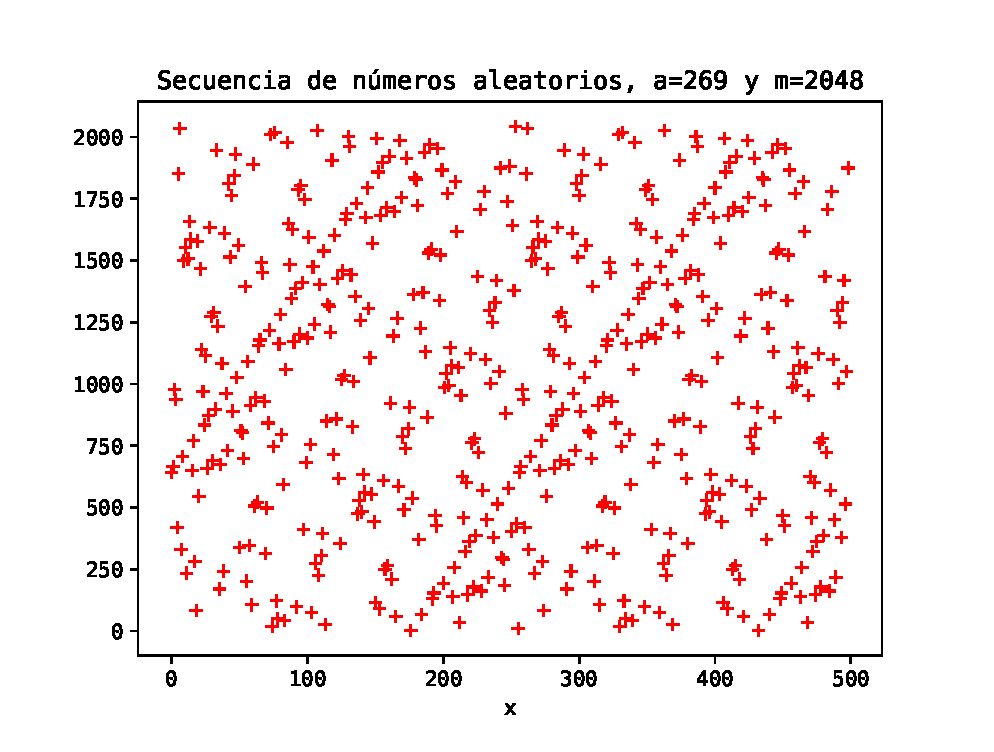
\includegraphics[scale=0.6]{Imagenes/Secuencia_aleatoria_02.eps}
\end{figure}
\end{frame}

\subsection{Funciones de python}

\begin{frame}
\frametitle{La librería \texttt{random}}
La librería \funcionazul{random} implementa generadores de números pseudoaleatorios para diversas distribuciones.
\\
\bigskip
\pause
Para números enteros, hay selección uniforme de un rango.
\end{frame}
\begin{frame}
\frametitle{La librería \texttt{random}}
Para las secuencias, hay una selección uniforme de un elemento aleatorio, una función para generar una permutación aleatoria de una lista \emph{in situ} y una función para el muestreo aleatorio sin reemplazo.
\end{frame}
\begin{frame}
\frametitle{La librería \texttt{random}}
Casi todas las funciones de la librería dependen de la función básica \funcionazul{random()}, que genera un número flotante aleatorio de manera uniforme en el rango semiabierto $[0.0, 1.0)$
\end{frame}
\begin{frame}
\frametitle{La librería \texttt{random}}
En \python{} se usa el algoritmo \textocolor{cobalt}{Mersenne Twister} como generador central. Produce números flotantes de precisión de $53$ bits y tiene un período de $2^{19937}-1$.
\end{frame}
\begin{frame}
\frametitle{Alcance del generador en \texttt{random}}
El algoritmo \textocolor{cobalt}{Mersenne Twister} es uno de los generadores de números aleatorios más probados que existen.
\\
\bigskip
\pause
Sin embargo, al ser completamente determinista, no es adecuado para todos los propósitos, y es completamente inadecuado para fines criptográficos.
\end{frame}
\begin{frame}
\frametitle{Funciones importantes}
Dentro de la librería \funcionazul{random} existen distintas funciones que podremos utilizar, basta con revisar la documentación disponible, para identificar los parámetros y la respuesta que devuelve.
\end{frame}
\begin{frame}
\frametitle{Funciones importantes}
Mencionaremos dos funciones:
\pause
\setbeamercolor{item projected}{bg=daffodil,fg=darkcoral}
\setbeamertemplate{enumerate items}{%
\usebeamercolor[bg]{item projected}%
\raisebox{1.5pt}{\colorbox{bg}{\color{fg}\footnotesize\insertenumlabel}}%
}
\begin{enumerate}[<+->]
\item \funcionazul{random.seed(a=None)}. Inicializa el generador de números aleatorios. Si no se especifica el valor de $a$, se utiliza el reloj del sistema. En caso de que $a$ sea un entero, se utilza directamente.
\item \funcionazul{random.random()}. Devuelve un número de punto flotante en el rango $[0.0, 1.0)$.
\end{enumerate}
\end{frame}
\begin{frame}
\frametitle{Ejemplo con \texttt{nprandom.seed(a)}}
Haremos un ejercicio en donde se van a generar tres secuencias de números con la función \funcionazul{nprandom.seed(a)}, cambiaremos el valor de la semilla y vamos a comparar los resultados en una gráfica.
\end{frame}
\begin{frame}[plain, allowframebreaks, fragile]
\frametitle{Código usando \texttt{seed()}}
\begin{lstlisting}[caption=Código con semilla]
import matplotlib.pyplot as plt
import random

def arreglonumeros(muestra=500, semilla=None):
    x = []
    random.seed(semilla)
    
    for i in range(muestra):
        nuevoValor = random.random()
        x.append(nuevoValor)
    
    return x

x1 = arreglonumeros()
x2 = arreglonumeros(semilla=500)
x3 = arreglonumeros(semilla=2018)

plt.figure(figsize=(8,5)) 
plt.plot(x1,'b+', label='seed = reloj sistema')
plt.plot(x2,'r+', label='seed = 500')
plt.plot(x3,'y+', label='seed = 2018')
plt.legend(loc='best')
plt.title('Secuencia de numeros aleatorios')
plt.xlabel('x')
plt.ylabel('y')
plt.show()
\end{lstlisting}
\end{frame}
\begin{frame}[fragile]
\frametitle{Gráfica obtenida}
\begin{figure}
  \centering
  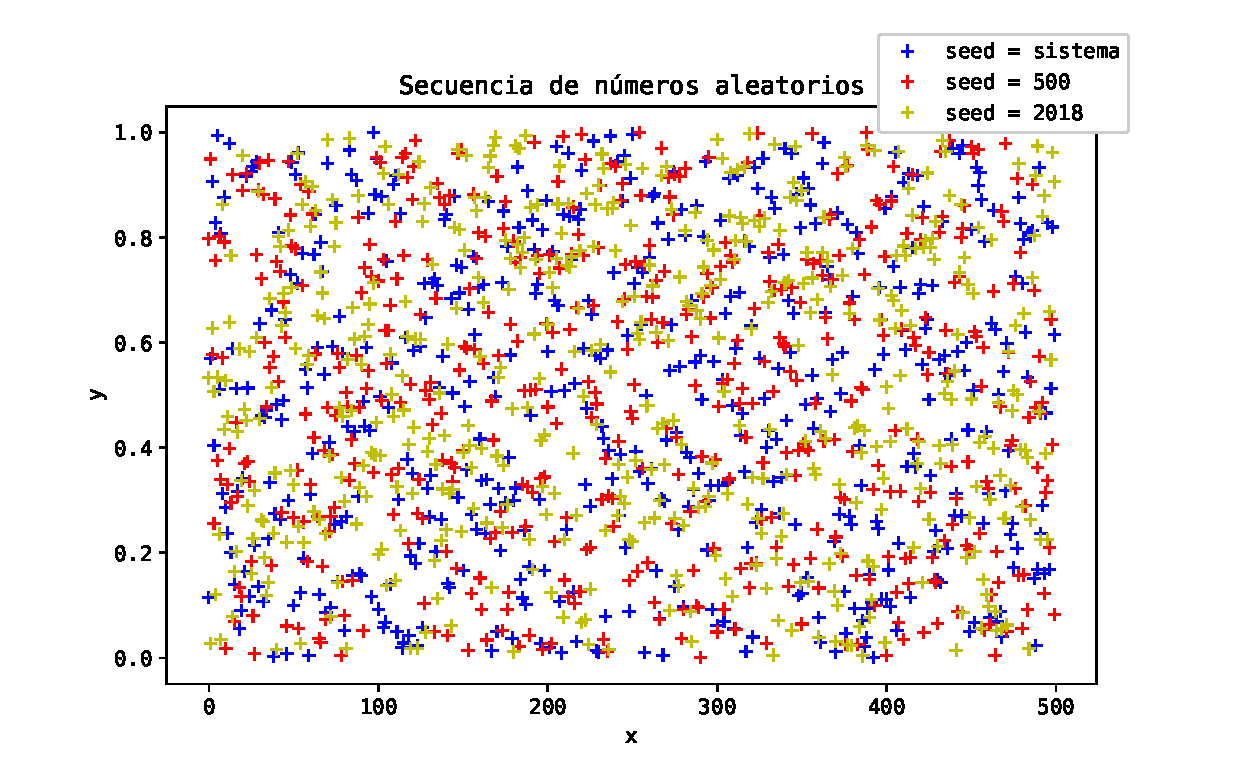
\includegraphics[scale=0.50]{Imagenes/Secuencia_aleatoria_04.eps}
\end{figure}
\end{frame}

\section{Decaimiento radiactivo}
\frame{\tableofcontents[currentsection, hideothersubsections]}
\subsection{Ejemplo}

\begin{frame}
\frametitle{El problema a estudiar}
El radioisótopo ${}^{208}$Tl (talio $208$) se desintegra a ${}^{208}$Pb estable (plomo $208$) con una vida media de $\SI{3.053}{\minute}$.
\end{frame}
\begin{frame}
\frametitle{Condiciones iniciales}
Supongamos que comenzamos con una muestra de $1000$ átomos de talio.
\\
\bigskip
\pause
\textocolor{darkmagenta}{Simulemos} la descomposición de estos átomos con el tiempo, imitando la aleatoriedad de esa descomposición utilizando números aleatorios.
\end{frame}
\begin{frame}
\frametitle{Hecho conocido}
En promedio, sabemos que el número $N$ de átomos en nuestra muestra disminuirá exponencialmente con el tiempo de acuerdo con la ecuación estándar de desintegración radiactiva:
\pause
\begin{align}
N (t) =  N (0) \, 2^{-\frac{t}{\tau}}
\label{eq:ecuacion_10_02}
\end{align}
donde $\tau$ es la vida media.
\end{frame}
\begin{frame}
\frametitle{Átomos que continuan}
Entonces, la fracción de átomos que quedan después del tiempo $t$ es:
\pause
\begin{align*}
\dfrac{N (t)}{N (0)} = 2^{-\frac{t}{\tau}}
\end{align*}
\pause
y la fracción que se ha desintegrado, que también es igual a la probabilidad $p (t)$ de que cualquier átomo en particular se haya desintegrado, es uno menos este número:
\pause
\begin{align}
p (t) = 1 - 2^{-\frac{t}{\tau}}
\label{eq:ecuacion_10_03}
\end{align}
\end{frame}
\begin{frame}
\frametitle{De la probabilidad}
Así, este número $p (t)$ representa la probabilidad de que un solo átomo se desintegre en un intervalo de tiempo de longitud $t$.
\end{frame}
\begin{frame}
\frametitle{Lo que queremos simular}
Simularemos la descomposición de nuestra muestra de $1000$ átomos dividiendo los átomos en dos conjuntos, uno de talio y otro de plomo.
\\
\bigskip
\pause
Inicialmente todos los átomos están en el conjunto de talio.
\end{frame}
\begin{frame}
\frametitle{Siguiente paso}
Dividiremos el tiempo en pasos de $1$ segundo cada uno y en cada paso de tiempo consideraremos a su vez cada átomo de talio y con la probabilidad dada por la ec. (10.3) decide si decae o no.
\end{frame}
\begin{frame}
\frametitle{Contando átomos de talio}
De esta forma calculamos el número total de átomos de talio que se desintegran en cada segundo, \pause luego restamos este número del total del conjunto de talio y lo sumamos al total del conjunto de plomo.
\end{frame}
\begin{frame}[allowframebreaks, fragile]
\frametitle{Código para la simulación}
\begin{lstlisting}[caption=Código para representar la desintegración radioactiva]
import matplotlib.pyplot as plt
from random import random
import numpy as np

NTl = 1000
NPb = 0
tau = 3.053*60
h = 1
p = 1 - 2**(-h/tau)
tmax = 1000

tpuntos = np.arange(0., tmax, h)
Tlpuntos = []
Pbpuntos = []

for i in tpuntos:
    Tlpuntos.append(NTl)
    Pbpuntos.append(NPb)
    decaimiento = 0
    
    for i in range(NTl):
        if random() < p:
            decaimiento += 1
    
    NTl -= decaimiento
    NPb += decaimiento

# Va la rutina de graficación
\end{lstlisting}
\end{frame}
\begin{frame}
\frametitle{Resultado obtenido}
\begin{figure}
    \centering
    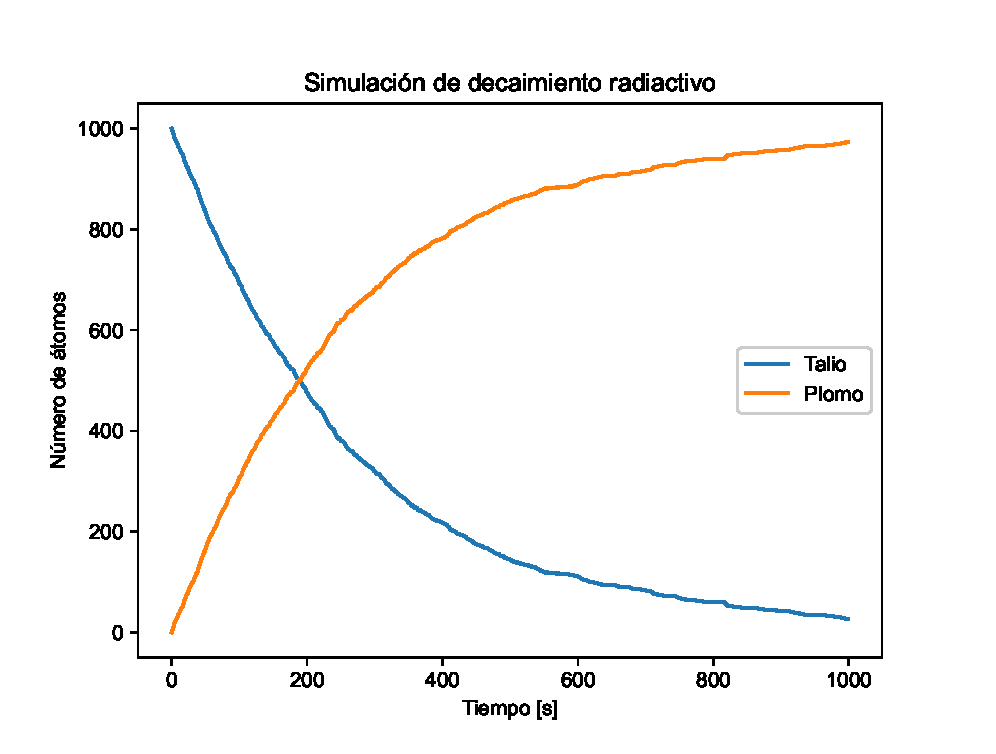
\includegraphics[scale=0.55]{Imagenes/plot_decaimiento_radiactivo_01.eps}
\end{figure}
\end{frame}
\begin{frame}
\frametitle{Interpretación}
El decaimiento exponencial general del talio claramente, pero también podemos ver una cierta cantidad de \enquote{ruido}, \pause ondulaciones aleatorias en las líneas, que surgen debido a la naturaleza inherentemente aleatoria del proceso de decaimiento.
\end{frame}
\begin{frame}
\frametitle{Interpretación}
Esta aleatoriedad no es capturada por el modelo exponencial estándar para la desintegración radiactiva, \pause pero puede ser capturada, como vemos aquí, por una simulación por computadora del proceso.
\end{frame}

\subsection{Ejercicio a cuenta}

\begin{frame}
\frametitle{Enunciado del ejercicio}
El isótopo ${}^{213}$Bi se descompone en ${}^{209}$Bi estable a través de una de dos rutas diferentes, con probabilidades y vidas medias como se muestra en la siguiente figura:
\end{frame}
\begin{frame}
\frametitle{Proceso de desintegración}
\begin{figure}
    \centering
    \begin{tikzpicture}[scale=0.8, font=\footnotesize]
        \draw (0, 0) rectangle (1.5, 1.5);
        \draw (2.5, -0.5) rectangle (4, -2);
        \draw (0, -2.5) rectangle (1.5, -4);
        \draw (0, -6) rectangle (1.5, -7);
        
        \node at (0.75, 1) {${}^{213}$Bi};
        \node at (0.75, 0.5) {$\SI{46}{\minute}$};

        \draw [-stealth, thick] (1.5, 0) -- (2.5, -0.5);
        
        \node at (3.3, -1) {${}^{209}$Tl};
        \node at (3.3, -1.5) {$\SI{2.2}{\minute}$};
        
        \draw [-stealth, thick] (0.72, 0) -- (0.72, -2.5);
        \draw [-stealth, thick] (2.5, -1.5) -- (1.3, -2.4);
        
        \node at (0.75, -3) {${}^{209}$Pb};
        \node at (0.75, -3.5) {$\SI{3.3}{\minute}$};
        
        \draw [-stealth, thick] (0.72, -4) -- (0.72, -6);
        
        \node at (0.75, -6.5) {${}^{209}$Bi};
        
        \node at (2.5, 0.5) {$2.09 \%$};
        \node at (-0.4, -1.3) {$97.91 \%$};

    \end{tikzpicture}
\end{figure}
\end{frame}
\begin{frame}
\frametitle{Aclaración importante}
Técnicamente, el ${}^{209}$Bi no es realmente estable, pero tiene una vida media de más de $\num{d19}$ años, mil millones de veces la edad del universo, por lo que bien podría serlo.
\end{frame}
\begin{frame}
\frametitle{A resolver en el ejercicio}
Comenzando con una muestra que consta de $10000$ átomos de ${}^{213}$Bi, simula la descomposición de los átomos como en el Ejercicio anterior, dividiendo el tiempo en segmentos de longitud $\delta t = \SI{1}{\second}$ cada uno y en cada paso haciendo lo siguiente:
\end{frame}
\begin{frame}
\frametitle{A resolver en el ejercicio}
\setbeamercolor{item projected}{bg=black,fg=white}
\setbeamertemplate{enumerate items}{%
\usebeamercolor[bg]{item projected}%
\raisebox{1.5pt}{\colorbox{bg}{\color{fg}\footnotesize\insertenumlabel}}%
}
\begin{enumerate}[<+->]
\item Para cada átomo de Pb a su vez, decidir al azar, con la probabilidad adecuada, si se desintegra o no. (La probabilidad se puede calcular a partir de la ecuación (\ref{eq:ecuacion_10_03}).) Cuenta el número total que se desintegra, réstalo del número de átomos de ${}^{209}$Pb y súmalo al número de átomos de ${}^{209}$Bi.
\seti
\end{enumerate}
\end{frame}
\begin{frame}
\frametitle{A resolver en el ejercicio}
\setbeamercolor{item projected}{bg=black,fg=white}
\setbeamertemplate{enumerate items}{%
\usebeamercolor[bg]{item projected}%
\raisebox{1.5pt}{\colorbox{bg}{\color{fg}\footnotesize\insertenumlabel}}%
}
\begin{enumerate}[<+->]
\conti
\item Ahora repite lo mismo para el ${}^{209}$Tl, excepto que los átomos en descomposición se restan del total de ${}^{209}$Tl y se suman al total de ${}^{209}$Pb.
\seti
\end{enumerate}
\end{frame}
\begin{frame}
\frametitle{A resolver en el ejercicio}
\setbeamercolor{item projected}{bg=black,fg=white}
\setbeamertemplate{enumerate items}{%
\usebeamercolor[bg]{item projected}%
\raisebox{1.5pt}{\colorbox{bg}{\color{fg}\footnotesize\insertenumlabel}}%
}
\begin{enumerate}[<+->]
\conti
\item Para el ${}^{213}$Bi la situación es más complicada: cuando un átomo de ${}^{213}$Bi se desintegra hay que decidir al azar con la probabilidad adecuada la ruta por la que se desintegra. Cuenta los números que decaen por cada ruta para luego sumar y restar según corresponda.
\seti
\end{enumerate}
\end{frame}
\begin{frame}
\frametitle{Punto importante}
Toma en cuenta que debes trabajar desde arriba en la cadena hasta la parte inferior, no de abajo para la parte superior, esto evita que el mismo átomo se desintegre dos veces sin darse cuenta en un solo paso.
\end{frame}
\begin{frame}
\frametitle{A resolver en el ejercicio}
\setbeamercolor{item projected}{bg=black,fg=white}
\setbeamertemplate{enumerate items}{%
\usebeamercolor[bg]{item projected}%
\raisebox{1.5pt}{\colorbox{bg}{\color{fg}\footnotesize\insertenumlabel}}%
}
\begin{enumerate}[<+->]
\conti
\item Lleva un registro del número de átomos de cada uno de los cuatro isótopos en todo momento durante $20000$ segundos y elabora una sola gráfica que muestre los cuatro números en función del tiempo en los mismos ejes.
\end{enumerate}
\end{frame}

% \section{La aguja de Buffon}
% \frame{\tableofcontents[currentsection, hideothersubsections]}
% \subsection{Planteamiento}

% \begin{frame}
% \frametitle{La aguja de Buffon}
% Resulta que $\pi$ también desempeña un papel importante en un experimento llamado \enquote{el problema de la aguja de Buffon}.
% \\
% \bigskip
% El cual buscar determinar la probabilidad de que una aguja de longitud $\ell$, arrojada aleatoriamente aterrice en medio o atravesando una serie de líneas paralelas en el suelo.
% \end{frame}
% \begin{frame}
% \begin{figure}
% 	\centering
% 	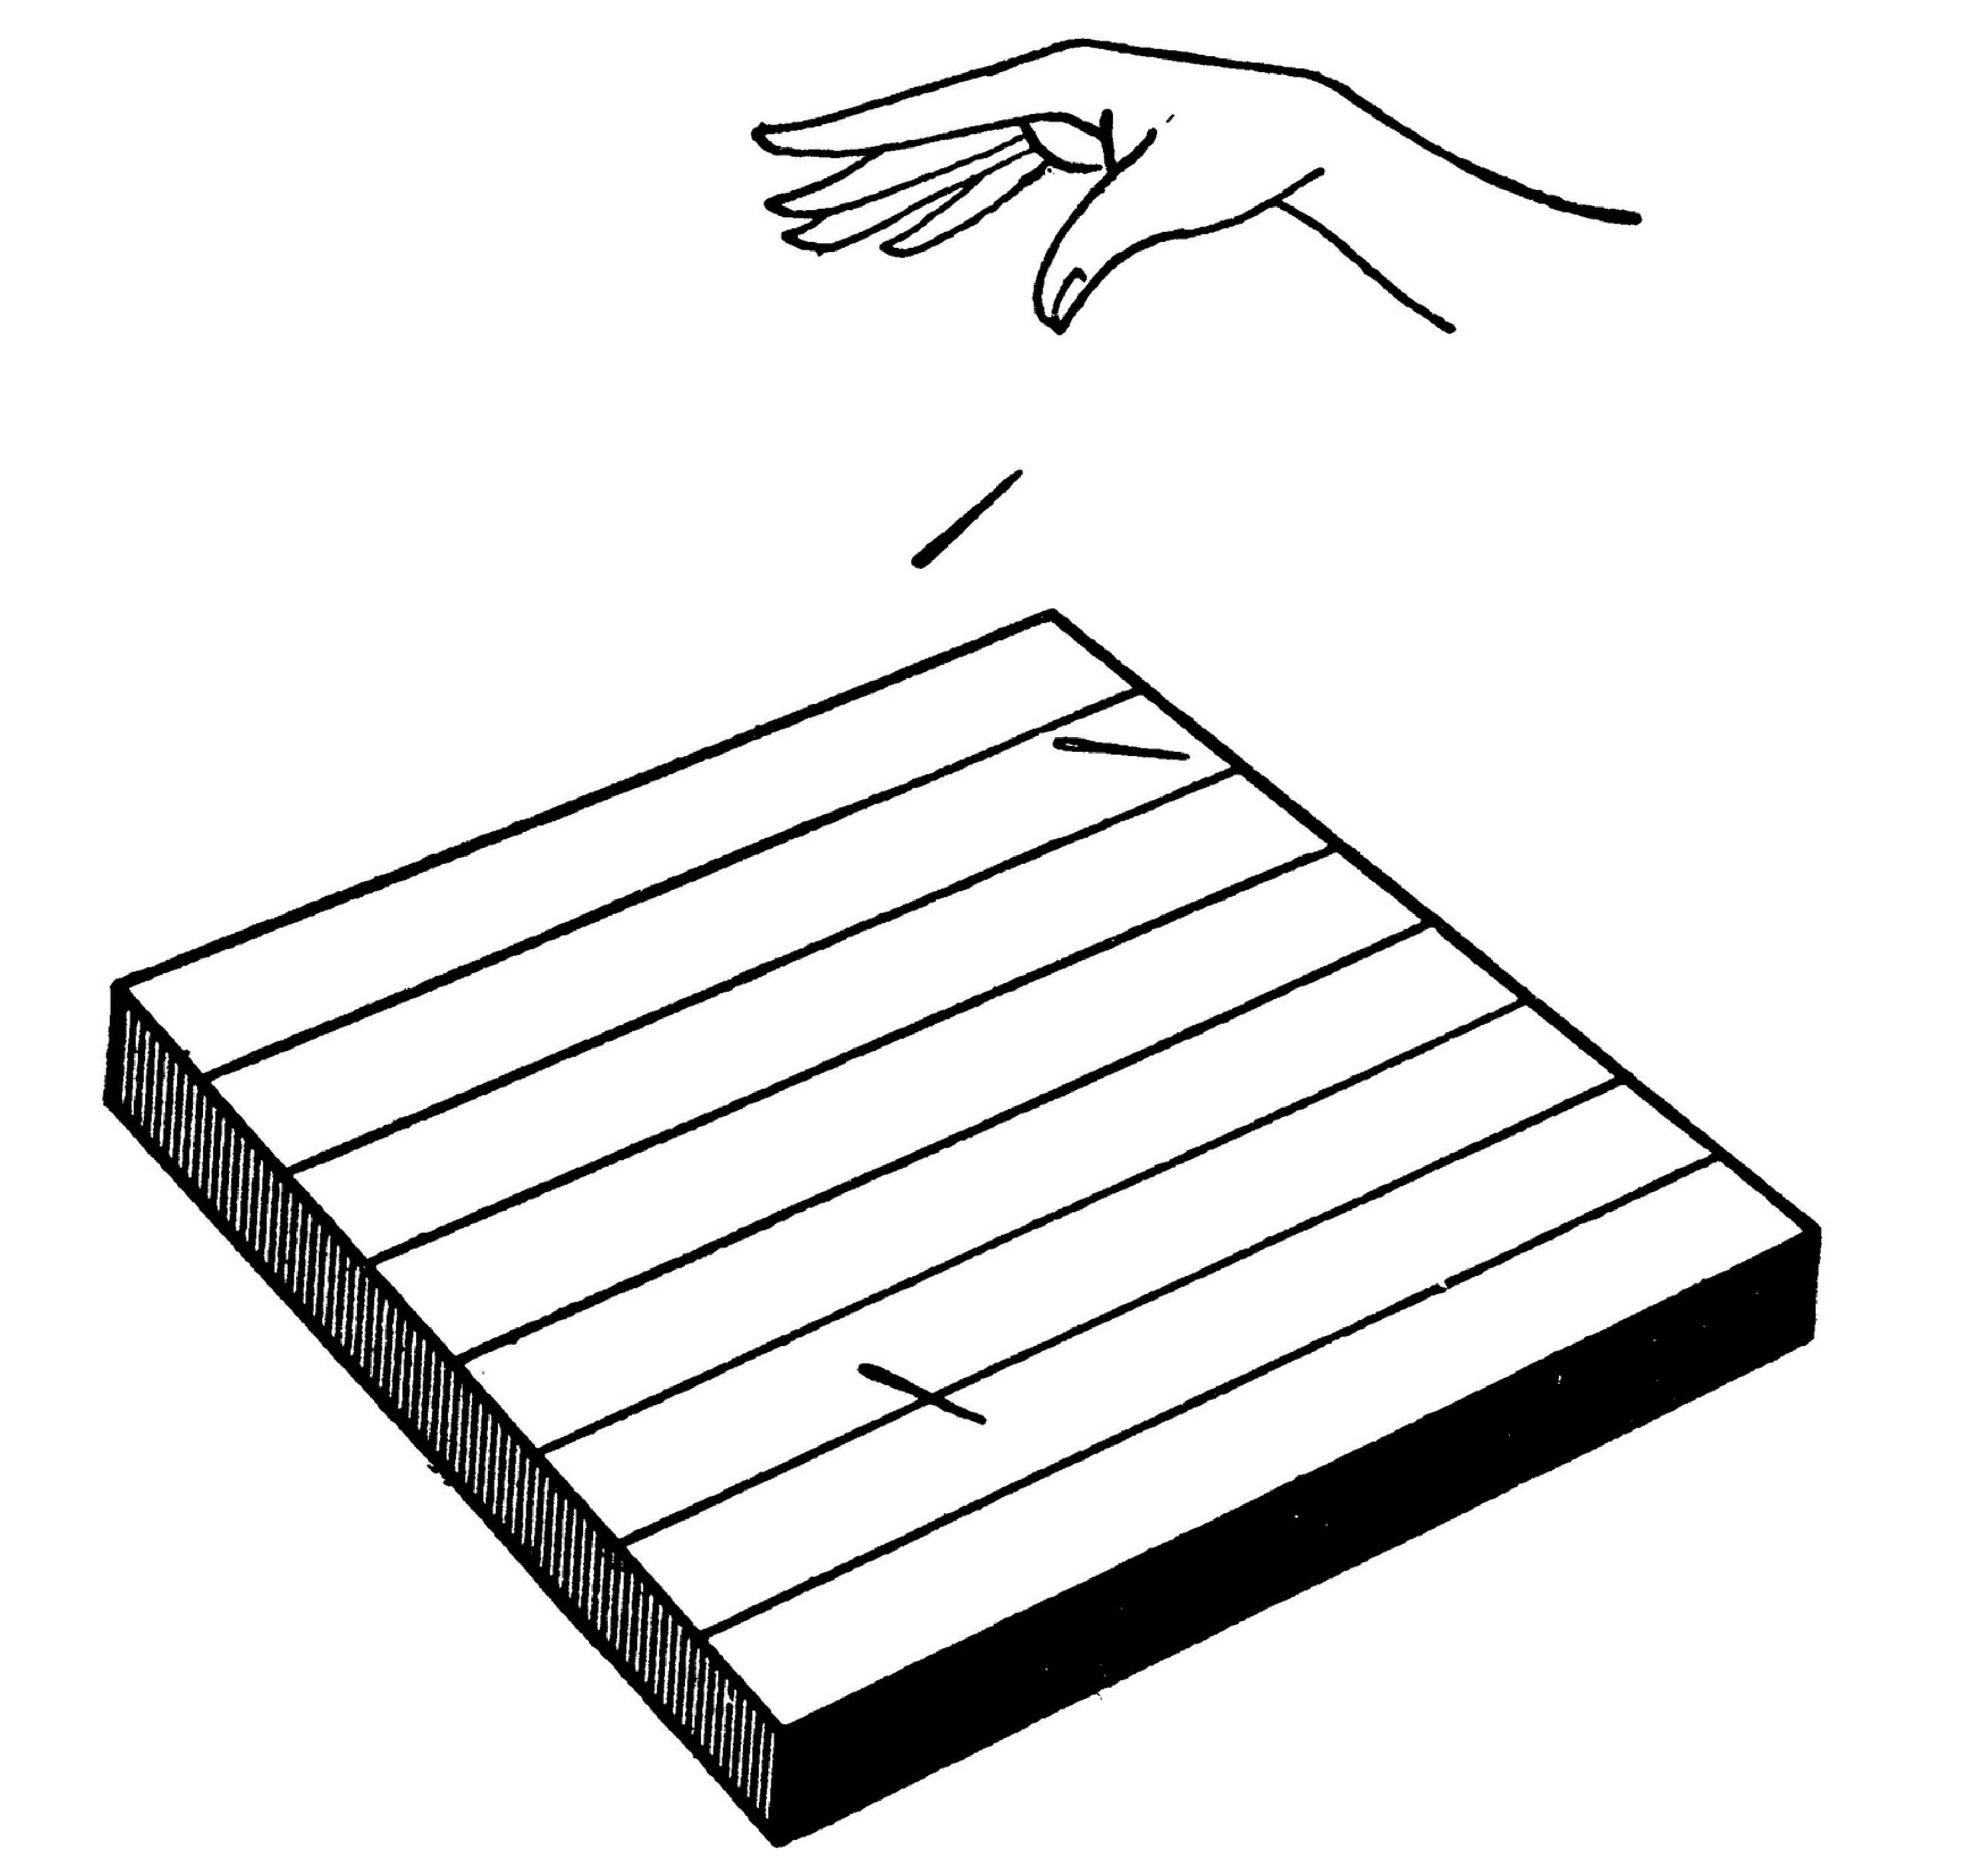
\includegraphics[scale=0.10]{aguja-de-buffon.eps}
% \end{figure}
% \end{frame}
% \begin{frame}
% \frametitle{La aguja de Buffon}
% Resulta que si la distancia entre las líneas paralelas es la misma que la longitud $\ell$ de la aguja lanzada, el número de veces que la aguja cae atravesando las líneas (luego de un gran número de lanzamientos), nos servirá para calcular el valor de $\pi$.
% \end{frame}
% \subsection{Aproximación al valor de $\pi$}
% \begin{frame}
% \frametitle{Aproximación al valor de $\pi$}
% De esa manera: 
% \[  \pi = \dfrac {2N}{A} \]
% siendo $N$ el número total de intentos y $A$ el número de veces que la aguja ha cruzado alguna línea.
% \end{frame}
% \begin{frame}
% \frametitle{Primer problema de tarea}
% Considera el caso en el que la longitud de la aguja es igual a la separación entre las rayas, es decir $\ell = h$.
% \\
% \bigskip
% Si la aguja cruza una línea de manera oblicua, es decir, existe un ángulo de inclinación con respecto a la línea, puedes deducir la relación a partir de la \enquote{función} que describe el caso de las agujas que tocan las líneas.
% \end{frame}
% \begin{frame}
% \frametitle{Segundo problema de tarea}
% Una vez que has deducido el problema, implementa en python un programa que calcule el valor aproximado de $\pi$, a partir del número de lanzamientos, y el número de agujas que cruzan una línea.
% \\
% \bigskip
% En las siguientes gráficas verás los resultados cuando se realiza el lanzamiento de $10^{2}, 10^{3}, 10^{4}, 10^{5}, 10^{6}$ agujas.
% \end{frame}
% % \begin{frame}
% % \frametitle{Configuración para el problema de la aguja}
% % \begin{figure}[fragile]
% % \begin{tikzpicture}{font=\small}
% % 	\draw [thick] (0, 0) -- (7,0);
% % 	\draw [thick] (0, 4) -- (7,4);
% % 	\draw [<->] (1,0) -- node[left] {Distancia entre líneas = 1}(1, 4);
% % \end{tikzpicture}
% % \end{figure}
% % \end{frame}
% \begin{frame}
% \frametitle{Solución con python}
% \begin{figure}
%   \centering
%   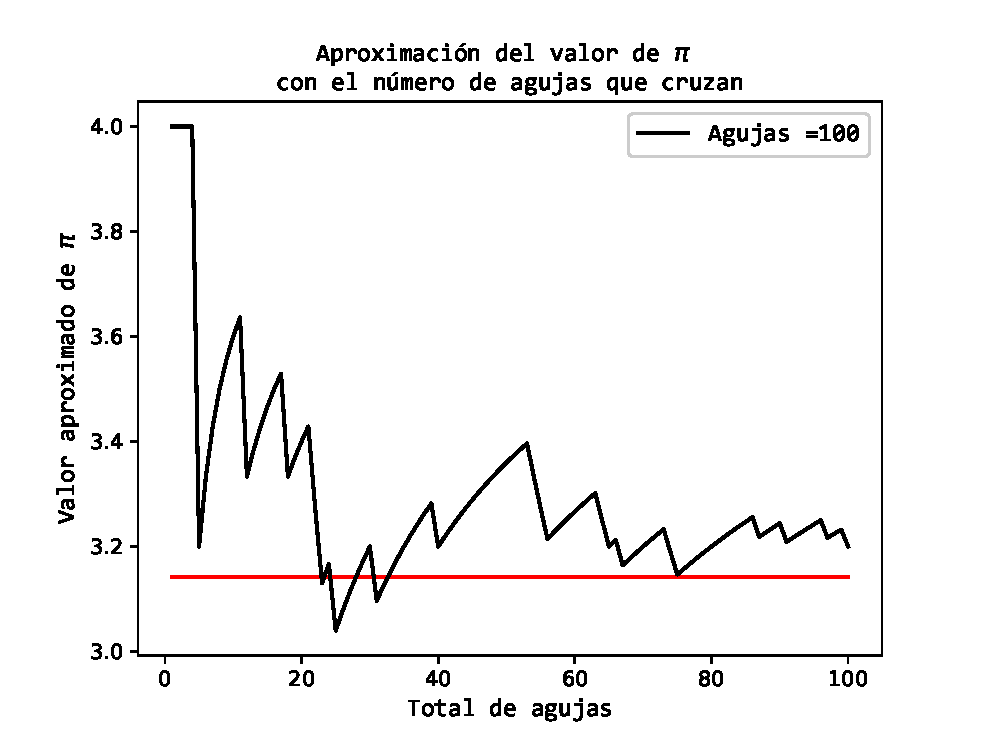
\includegraphics[scale=0.6]{aproximacionPi_100.eps}
% \end{figure}
% \end{frame}
% \begin{frame}
% \frametitle{Solución con python}
% \begin{figure}
%   \centering
%   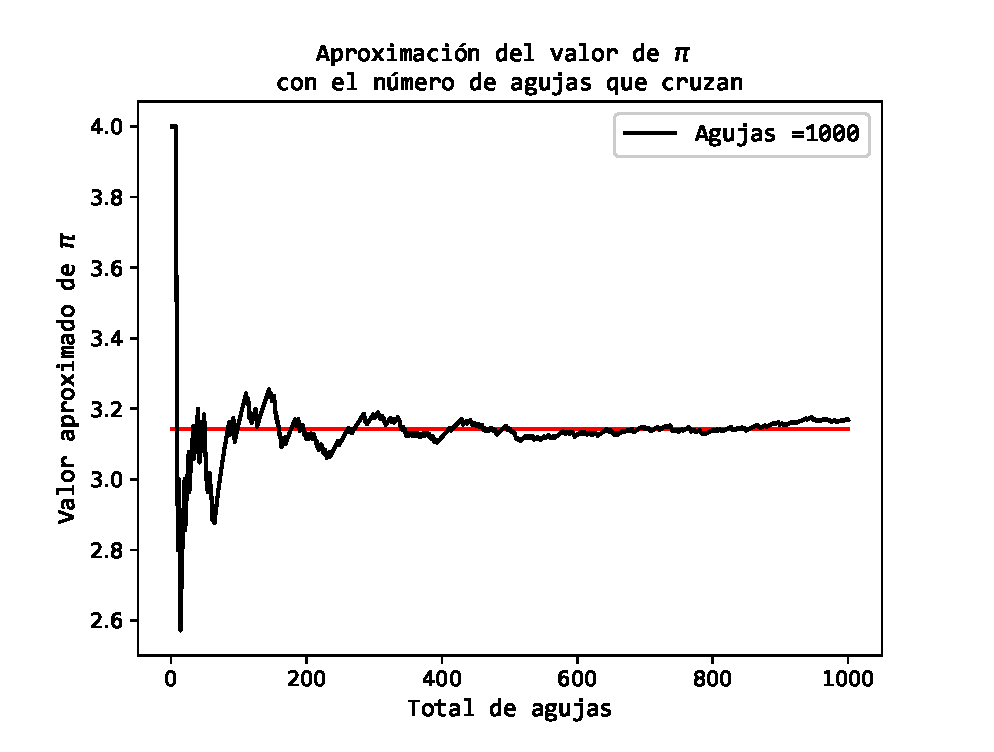
\includegraphics[scale=0.6]{aproximacionPi_1000.eps}
% \end{figure}
% \end{frame}
% \begin{frame}
% \frametitle{Solución con python}
% \begin{figure}
%   \centering
%   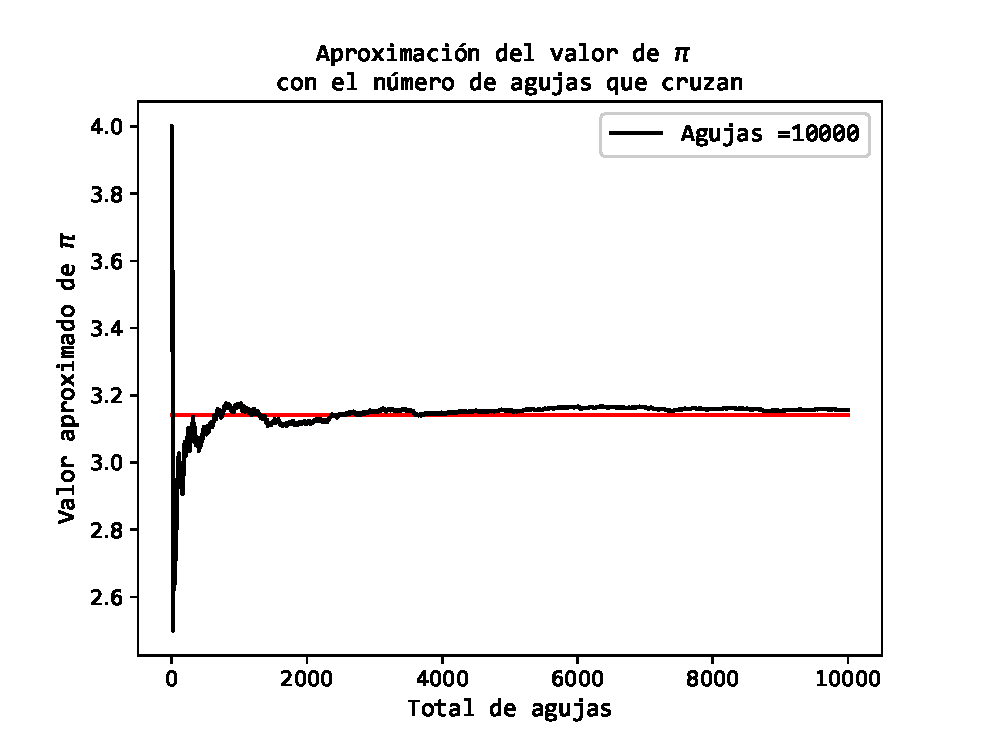
\includegraphics[scale=0.6]{aproximacionPi_10000.eps}
% \end{figure}
% \end{frame}
% \begin{frame}
% \frametitle{Solución con python}
% \begin{figure}
%   \centering
%   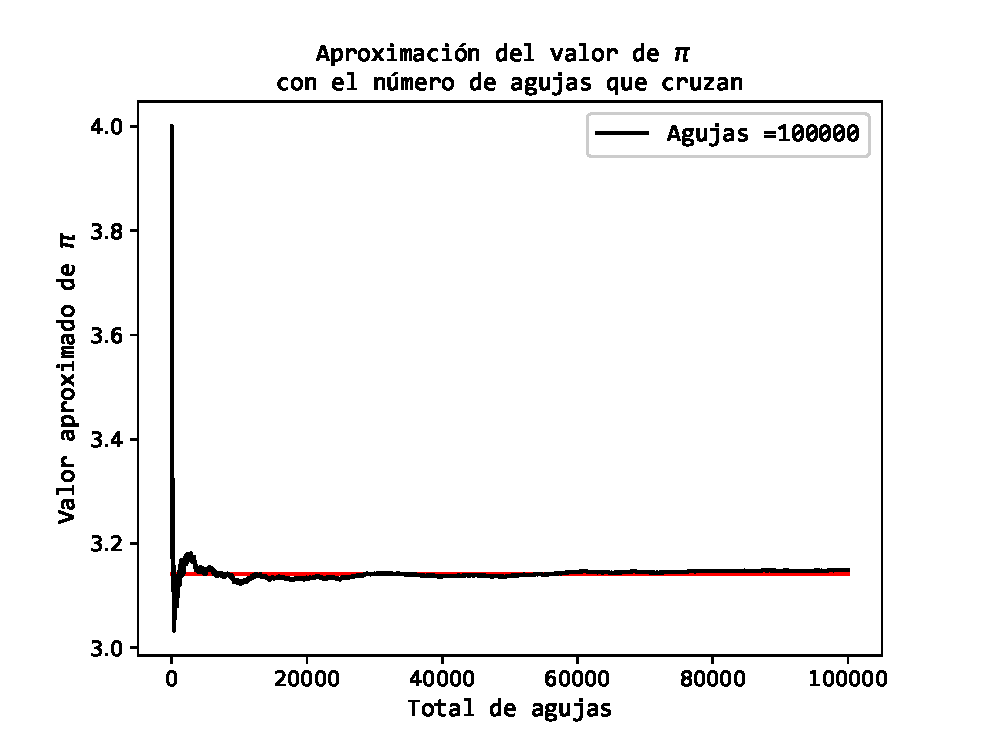
\includegraphics[scale=0.6]{aproximacionPi_100000.eps}
% \end{figure}
% \end{frame}
% \begin{frame}
% \frametitle{Solución con python}
% \begin{figure}
%   \centering
%   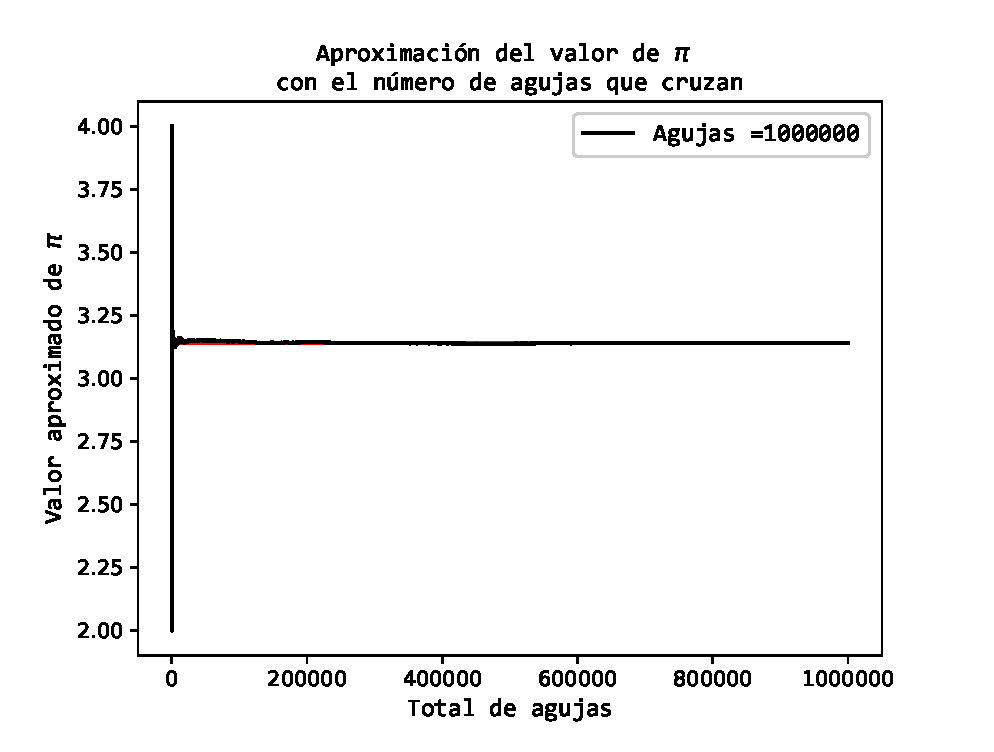
\includegraphics[scale=0.6]{aproximacionPi_1000000.eps}
% \end{figure}
% \end{frame}

\section{Aplicaciones Monte Carlo}
\frame{\tableofcontents[currentsection, hideothersubsections]}
\subsection{Integración Monte Carlo}

\begin{frame}
\frametitle{Integración Monte Carlo}
Una de las primeras aplicaciones con el uso de números aleatorios ha sido el cálculo numérico de integrales, es decir, un problema no aleatorio (determinista).
\\
\bigskip
\pause
Veamos un primer método para calcular:
\begin{align*}
\scaleint{6ex}_{\bs a}^{b} f (x) \; \dd{x}
\end{align*}
\end{frame}
\begin{frame}
\frametitle{Integración estándar Monte Carlo}
Sea $x_{1}, x_{2}, \ldots, x_{n}$ la secuencia de números aleatorios uniformemente distribuidos entre $a$ y $b$.
\\
\bigskip
\pause
Entonces
\begin{align}
(b - a) \; \dfrac{1}{n} \; \nsum_{i=1}^{n} f (x_{i})
\label{eq:ecuacion_08_07}
\end{align}
\end{frame}
\begin{frame}
\frametitle{Aproximación a la integral}
Es una aproximación a la integral:
\begin{align*}
\scaleint{6ex}_{a}^{b} f (x) \dd{x}
\end{align*}
Este método se denomina generalmente \textocolor{darkred}{integración de Monte Carlo}.
\end{frame}
\begin{frame}
\frametitle{Aproximación a la integral}
Es fácil de interpretar la ec. (\ref{eq:ecuacion_08_07}): \pause Un resultado bien conocido del cálculo es que la integral de una función $f$ sobre $[a, b]$ es igual al valor medio de $f$ sobre $[a, b]$ multiplicado por la longitud del intervalo, $(b - a)$.
\end{frame}
\begin{frame}
\frametitle{Aproximación a la integral}
Si aproximamos el valor medio de $f (x)$ por la media de $n$ evaluaciones de la función distribuidas al azar $f (x_{i})$, obtenemos el método de integración.
\end{frame}
\begin{frame}
\frametitle{El módulo \funcionazul{moduloAleatorio}}
Todas las funciones que revisaremos, deben de quedar contenidas en el módulo \funcionazul{moduloAleatorio}, para que se manden llamar cuando se requiera.
\\
\bigskip
\pause
Recuerda que la modularidad nos organiza y simplifica el trabajo.
\end{frame}
\begin{frame}[allowframebreaks, fragile]
\frametitle{Estimado la integral con python}
Podemos implementar la ec. (\ref{eq:ecuacion_08_07}) en una pequeña función de \python:
\begin{lstlisting}[caption=Función para aproximar la integral]
import random

def intMC(f, a, b, n):
    s = 0
    for i in range(n):
        x = random.uniform(a, b)
        s += f(x)
        
    I = (float(b-a)/n) * s
    return I
\end{lstlisting}
\end{frame}
\begin{frame}[fragile]
\frametitle{Versión más rápida del código}
Normalmente se necesita un valor de $n$ grande para obtener buenos resultados con este método, por lo que una versión vectorizada más rápida de la función anterior es útil:
\end{frame}
\begin{frame}[plain, fragile]
\frametitle{Versión más rápida del código}
\begin{lstlisting}[caption=Función vectorizada para la aproximación de la integral]
import numpy as np

def intvecMC(f, a, b, n):
    x = np.random.uniform(a, b, n)
    s = np.sum(f(x))
    I = (float(b-a)/n) * s

    return I
\end{lstlisting}
\end{frame}
\begin{frame}
\frametitle{Ejemplo}
Vamos a probar el método de integración de Monte Carlo en una función simple, sea $f (x) = 2 + 3 \: x$, y calculemos la integral en $[1, 2]$.
\\
\bigskip
\pause
La mayoría de los otros métodos de integración numérica resolverán exactamente esa función lineal, independientemente del número de evaluaciones de la función.
\end{frame}
\begin{frame}
\frametitle{Ejemplo}
Este no es el caso de la integración de Monte Carlo. 
\\
\bigskip
\pause
Sería interesante ver cómo la calidad de la aproximación de Monte Carlo se incrementa, conforme crece el valor de $n$.
\end{frame}
\begin{frame}
\frametitle{Ejemplo}
Para graficar la evolución de la aproximación con la integral, debemos almacenar los valores intermedios $I$, por lo que debemos de modificar el código:
\end{frame}
\begin{frame}[plain, fragile]
\begin{lstlisting}[caption=Código modificado para el ejercicio]
def int2MC(f, a, b, n):
    # se guardan las aproximaciones intermedias de la integral en el arreglo I,
    # donde I[k-1] es k veces la funcion evaluada
    s = 0

    I = np.zeros(n)

    for k in range(1, n+1):
        x = np.random.uniform(a, b)
        s += f(x)
        I[k-1] = (float(b-a)/k) * s
    return I
\end{lstlisting}
\end{frame}
\begin{frame}
\frametitle{Consideraciones para la solución}
Toma en cuenta que hacemos que $k$ vaya de $1$ a $n$ mientras que los índices en $I$, como de costumbre, van de $0$ a $n-1$.
\end{frame}
\begin{frame}
\frametitle{Consideraciones para la solución}
Dado que $n$ puede ser muy grande, el arreglo $I$ puede consumir más memoria de lo que tenemos disponible en la computadora.
\\
\bigskip
\pause
Por lo tanto, decidimos almacenar sólo cada $N$ valores de la aproximación. 
\end{frame}
\begin{frame}[plain, fragile]
\frametitle{Consideraciones para la solución}
El determinar si un valor debe ser almacenado o no puede ser calculado por la función \texttt{mod}:
\begin{lstlisting}[caption=Almacenamiento de valores]
for k in range(1, n+1):
    if k % N == 0:
    	#se guarda
\end{lstlisting}
Es decir, cada vez que $k$ se divide $N$ sin ningún residuo, almacenamos el valor.
\end{frame}
\begin{frame}[allowframebreaks, fragile]
\frametitle{Código completo}
\begin{lstlisting}[caption=Código completo para el ejercicio]
def int3MC(f, a, b, n, N=100):
    s = 0
    Ivalores = []
    kvalores = []
    
    for k in range(1, n+1):
        x = np.random.uniform(a, b)
        s += f(x)
        if k % N == 0:
            I = (float(b-a)/k) * s
            Ivalores.append(I)
            kvalores.append(k)
    
    return kvalores, Ivalores
\end{lstlisting}
\end{frame}
\begin{frame}[plain, fragile]
\frametitle{Estimación del error}
Ahora podemos revisar el error que se genera al usar la función:
\begin{lstlisting}[caption=Estimación del error del procedimiento]
def f(x):
    return 2 + 3*x

k, I = int3MC(f, 1, 2, 1000000, N=10000)

# evalua el error absoluto
\end{lstlisting}
\end{frame}
\begin{frame}[fragile]
\frametitle{Gráfica del error vs $N$}
\begin{figure}
	\centering
	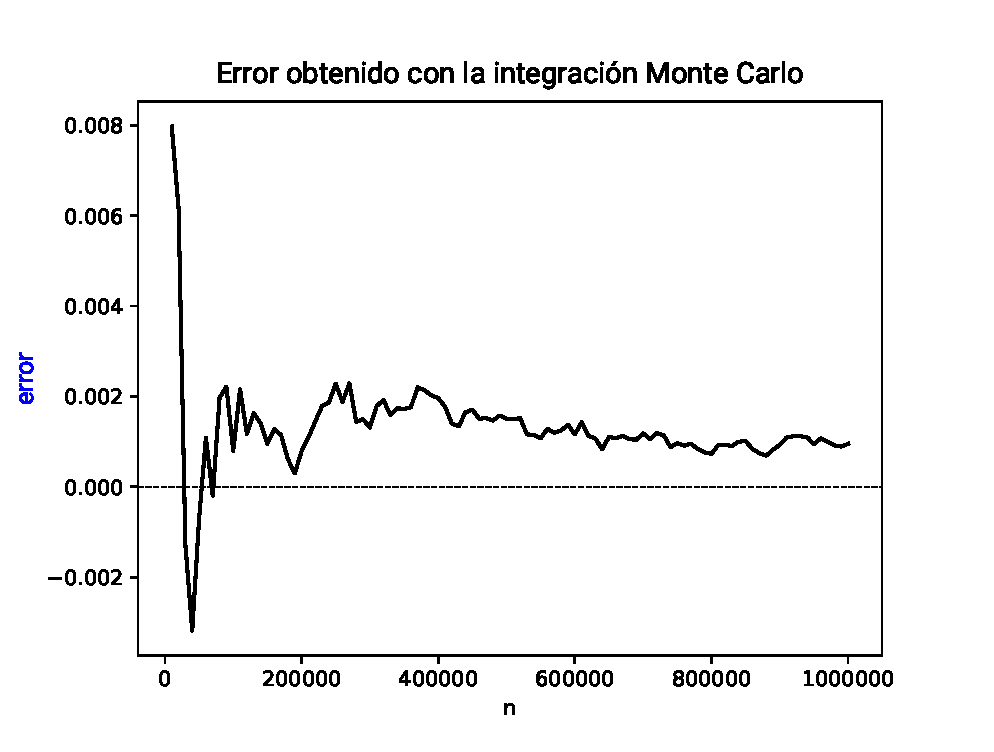
\includegraphics[scale=0.55]{Imagenes/integracionMC01_2017.eps}
	%\caption{Convergencia de la integración de Monte Carlo para $f(x)$}
\end{figure}
\end{frame}
\begin{frame}
\frametitle{Velocidad de convergencia}
Para funciones de una variable, el método (\ref{eq:ecuacion_08_07}) requiere de muchos puntos y es ineficiente comparado con otras reglas de integración.
\\
\bigskip
\pause
La mayoría de las reglas de integración tienen un error que se reduce mientras se incrementa $n$, normalmente de la manera $n^{-r}$ para un $r > 0$.
\end{frame}
\begin{frame}
\frametitle{Velocidad de convergencia}
Para la regla del trapecio, $r = 2$, mientras que para la integración de Monte Carlo $r = 1/2$
\\
\bigskip
\pause
Esto significa que este método converge muy lentamente en comparación con la regla del trapecio.
\end{frame}

\subsection{Integración en varias variables}

\begin{frame}
\frametitle{Integración en varias variables}
Sin embargo, para funciones de varias variables, la integración de Monte Carlo en espacios de dimensiones mayores supera completamente a métodos como la regla del trapecio y la regla de Simpson.
\end{frame}
\begin{frame}
\frametitle{Mejoras para el cálculo de la integral}
Existen diferentes maneras de mejorar el rendimiento de la ec. (\ref{eq:ecuacion_08_07}), básicamente por ser \enquote{aplicados} al momento de graficar los números aleatorios, conocidas como técnicas de reducción de la varianza.
\end{frame}

\subsection{Calculando áreas con puntos aleatorios}

\begin{frame}
\frametitle{Calculando áreas con puntos aleatorios}
Pensemos en alguna región geométrica $G$ en el plano y una caja circundante $B$ con geometría $[x_{L}, x_{H}] \times [y_{L}, y_{H}]$.
\\
\bigskip
\pause
Una forma de calcular el área de $G$ es dibujar $N$ puntos aleatorios dentro de $B$ y contar cuántos de ellos $M$, están dentro de $G$.
\end{frame}
\begin{frame}
\frametitle{Puntos dentro de la región}
El área de $G$ es entonces la fracción $M/N$ (fracción de $G$ en el área de $B$) veces el área de $B$, $(x_{H} - x_{L})(y_{H} - y_{L})$.
\end{frame}
\begin{frame}
\frametitle{Puntos dentro de la región}
De forma diferente, este método es una especie de juego de dardos en el que se cuentan los que caen dentro de $G$, si cada lanzamiento llega de manera uniforme dentro de $B$.
\end{frame}
\begin{frame}
\frametitle{Calculando una integral}
Veamos cómo será la expresión para calcular la integral:
\pause
\begin{align*}
\scaleint{6ex}_{\bs a}^{b} f (x) \: \dd{x}
\end{align*}
Como nota relevante, consideremos que esta integral es el área debajo de la curva $y = f (x)$ y sobre el eje $x$, entre $x = a$ y $x = b$.
\end{frame}
\begin{frame}
\frametitle{Calculando una integral}
Introducimos un rectángulo $B$, tal que:
\begin{align*}
B = \{ (x, y) \vert a \leq x \leq b, \hspace{0.3cm} 0 \leq y \leq m \}
\end{align*}
donde $m \leq \max_{x \in [a, b]} \; f (x)$
\end{frame}
\begin{frame}
\frametitle{Calculando una integral}
El algoritmo para calcular el área bajo la curva se basa en dibujar $N$ puntos aleatorios dentro de $B$ y contar cuántos de ellos, $M$, están por encima del eje $x-y$  y cuántos por debajo de la curva $y = f (x)$.
\end{frame}
\begin{frame}
\frametitle{Método del dardo}
\begin{figure}
	\centering
	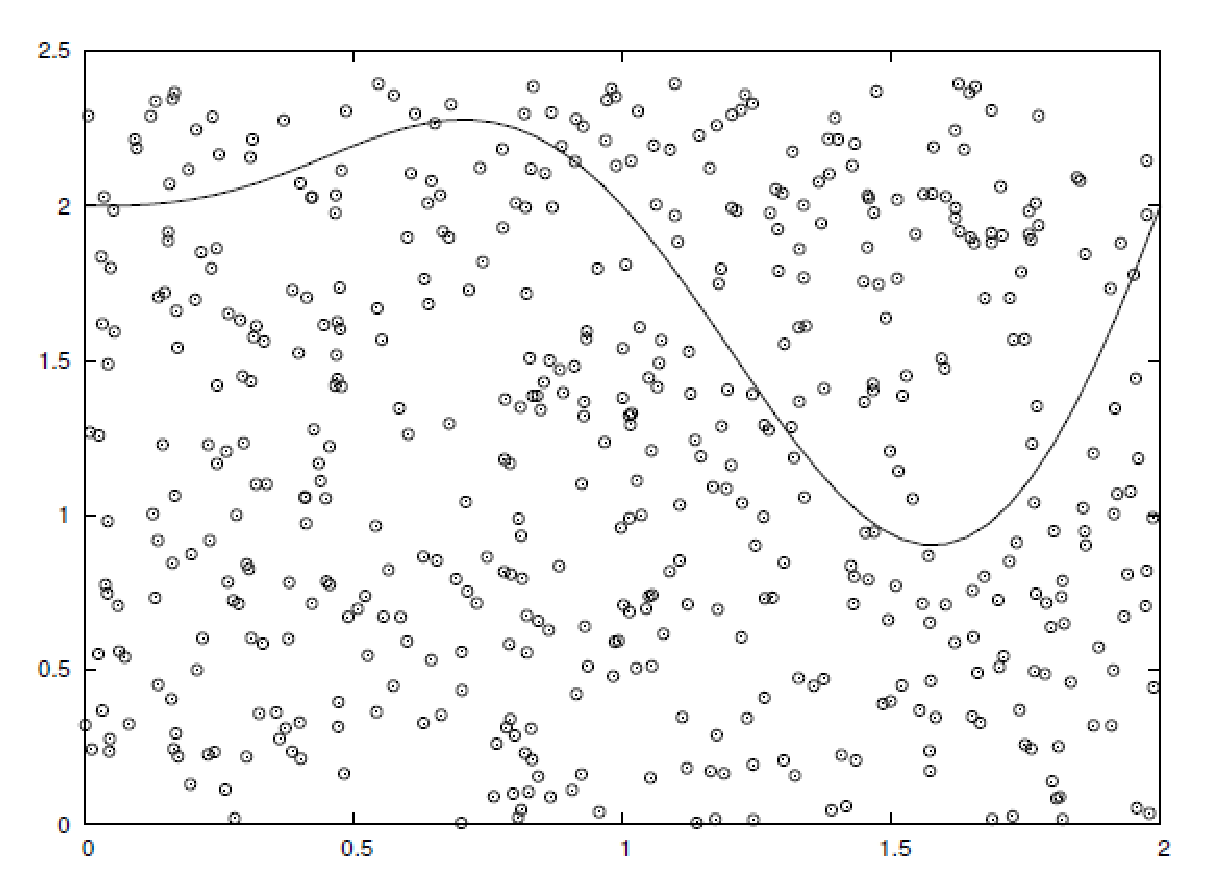
\includegraphics[scale=0.4]{Imagenes/integracionCaja.eps}
	\caption{\tiny{Cuando $M$ de $N$ puntos aleatorios en el rectángulo $[0, 2] \times [0, 2.4]$ se encuentran bajo la curva, el área bajo la curva se estima como la fracción $M / N$ del área del rectángulo.}}
\end{figure}
\end{frame}
\begin{frame}
\frametitle{Valor de la integral}
El área o el valor de la integral se estima por la expresión:
\pause
\begin{align*}
\dfrac{M}{N} \: m \: (b - a)
\end{align*}
\end{frame}
\begin{frame}[allowframebreaks, fragile]
\frametitle{Código para la integral}
\begin{lstlisting}[caption=Código para el método del dardo]
def intareaMC(f, a, b, n, m):
    porDebajo = 0 
    for i in range(n):
        x = random.uniform(a, b)
        y = random.uniform(0, m)
        if y <= f(x):
            porDebajo += 1
    area = porDebajo/float(n) * m * (b - a)
    
    return area
\end{lstlisting}
\end{frame}
\begin{frame}[fragile]
\frametitle{Cantidad de números aleatorios}
Toma en cuenta que este método opera con el doble de números aleatorios que el método anterior.
\\
\bigskip
\pause
Una implementación vectorizada del código sería la siguiente:
\end{frame}
\begin{frame}[allowframebreaks, fragile]
\frametitle{Listado en python}
\begin{lstlisting}[caption=Método del dardo en modo vectorizado]
def intareavecMC(f, a, b, n, m):
    x = random.uniform(a, b, n)
    y = random.uniform(0, m, n)
    porDebajo = np.sum(y < f(x))
    area = porDebajo/float(n) * m * (b - a)
    
    return area
\end{lstlisting}
\end{frame}
\begin{frame}
\frametitle{Cantidad de números aleatorios}
Podemos ejecutar el código para un conjunto de 2 millones de números al azar, la versión de bucle sencillo no es tan lenta.
\\
\bigskip
\pause
Sin embargo, si necesita que la integración se repita muchas veces dentro de otro cálculo, puede ser importante la eficacia superior de la versión vectorizada.
\end{frame}
\begin{frame}[allowframebreaks, fragile]
\frametitle{Código completo}
\begin{lstlisting}[caption=Función para el método del dardo]
def int3areaMC(f, a, b, n, m, N=1000):
    Ivalores = []
    kvalores = []
    porDebajo = 0
    
    for k in range(1, n+1):
        x = np.random.uniform(a, b)
        y = np.random.uniform(0, m)
        
        if y <= f(x):
            porDebajo += 1
        
        area = porDebajo/float(k) * m * (b-a)
        
        if k % N == 0:
            I = area
            Ivalores.append(I)
            kvalores.append(2 * k)
    
    return kvalores, Ivalores
\end{lstlisting}
\end{frame}
\begin{frame}
\frametitle{Implementación del código}
Al contar con los elementos necesarios, podemos implementar el código completo para estimar el valor de la integral a partir de generar puntos aleatorios.
\\
\bigskip
\pause
Haremos una estimación del tiempo que tarda en resolverse el problema usando el bucle y la versión vectorizada.
\end{frame}
\begin{frame}
\frametitle{La librería \funcionazul{time}}
La librería \funcionazul{time} proporciona un conjunto de funciones para registrar el tiempo en el equipo de cómputo.
\\
\bigskip
\pause
Revisa la documentación de la librería, ya que tiene como punto particular el hecho de medir el tiempo a partir del 1 de enero de 1970, al momento actual en el equipo.
\end{frame}
\begin{frame}
\frametitle{Para medir un intervalo}
Para el ejercicio que haremos, se requiere medir un intervalo de tiempo entre dos eventos, por lo que no es necesario hacer alguna conversión de tiempo.
\\
\bigskip
\pause
La función \funcionazul{time.process\_time()} hará el registro del tiempo en el equipo, para el intervalo, basta con que hagamos un segundo registro y tomar la diferencia entre éstos.
\end{frame}
\begin{frame}[allowframebreaks, fragile]
\begin{lstlisting}[caption=Implementación del código]
def f(x):
    return 2 + 3 * x

a = 1; b = 2; n = 1000000; N = 10000; fmax = f(b)

t0 = time.process_time()

valor1 = intareaMC(f, a, b, n, fmax)
print('Integral = {0:}'.format(valor1))
print('Error: {0:1.5e}'.format(error(valor1)))

t1 = time.process_time()

print('Tiempo en bucle: {0} segundos'.format(t1 - t0))

valor2 = intareavecMC(f, a, b, n, fmax)
print('\nIntegral = {0:}'.format(valor2))
print('Error: {0:1.5e}'.format(error(valor2)))

t2 = time.process_time()
print('Tiempo en vectorizada: {0} segundos'.format(t2 - t1))

print ('\nFraccion bucle/vectorizada: {0:}'.format((t1 - t0)/(t2 - t1)))

k, I = int3areaMC(f, a, b, n, fmax, N)

print('\nIntegral = {0:}'.format(I[-1]))
print('Error: {0:1.5e}'.format(error(I[-1])))
\end{lstlisting}
\end{frame}
\begin{frame}
\frametitle{Graficando los puntos}
A continuación se presenta una gráfica con los puntos aleatorios debajo de la función y por arriba de ésta.
\\
\bigskip
\pause
No tendrás problema para implementar el código necesario para las gráficas. \pause \textocolor{ao}{Es un ejercicio a cuenta del examen: completar el código que genere las gráficas}
\end{frame}
\begin{frame}
\frametitle{Gráfica de la función inicial}
\begin{figure}
	\centering
	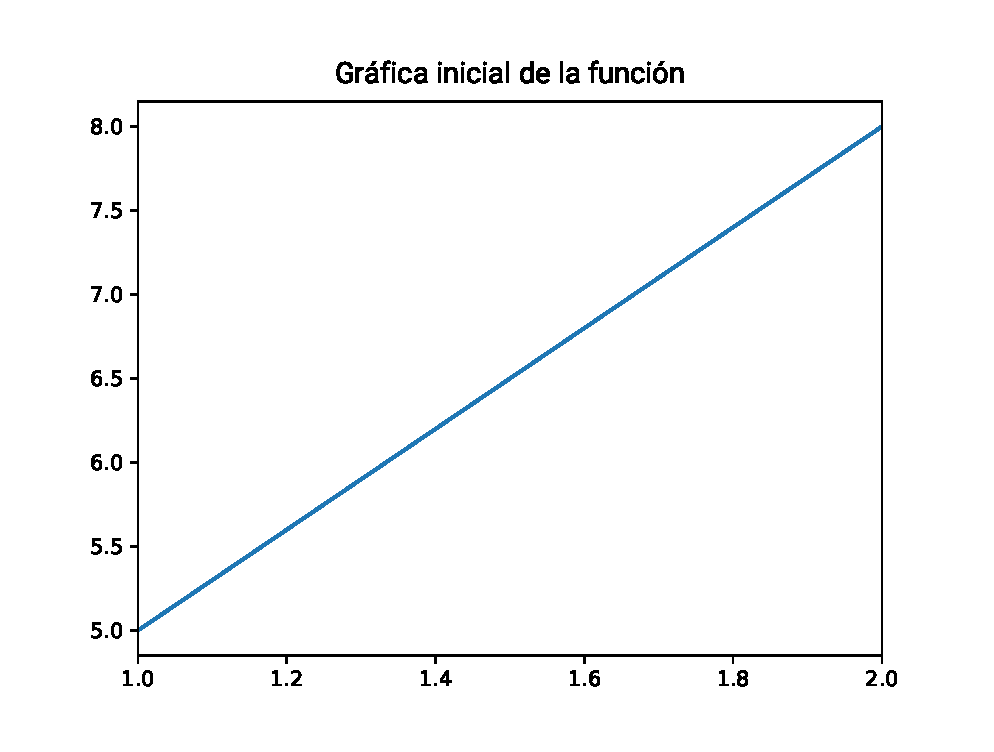
\includegraphics[scale=0.55]{Imagenes/area_puntos_01.eps}
\end{figure}
\end{frame}
\begin{frame}
\frametitle{Puntos aleatorios por arriba y por abajo}
\begin{figure}
    \centering
    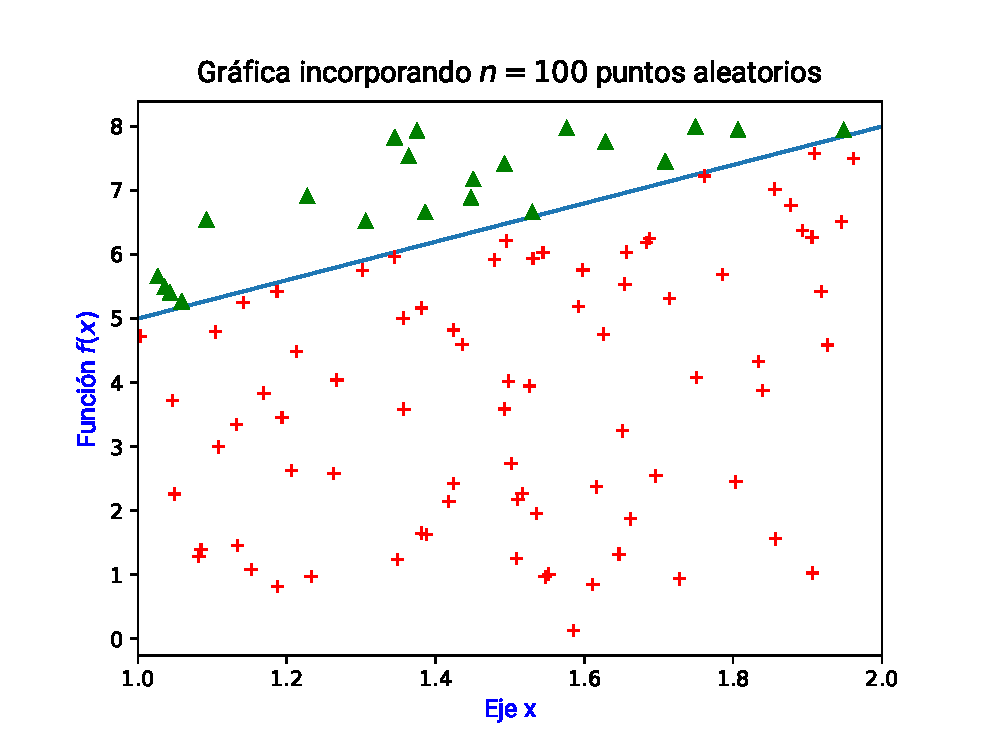
\includegraphics[scale=0.55]{Imagenes/area_puntos_02.eps}
\end{figure}
\end{frame}
\begin{frame}
\frametitle{Gráfica cubriendo el área}
\begin{figure}
    \centering
    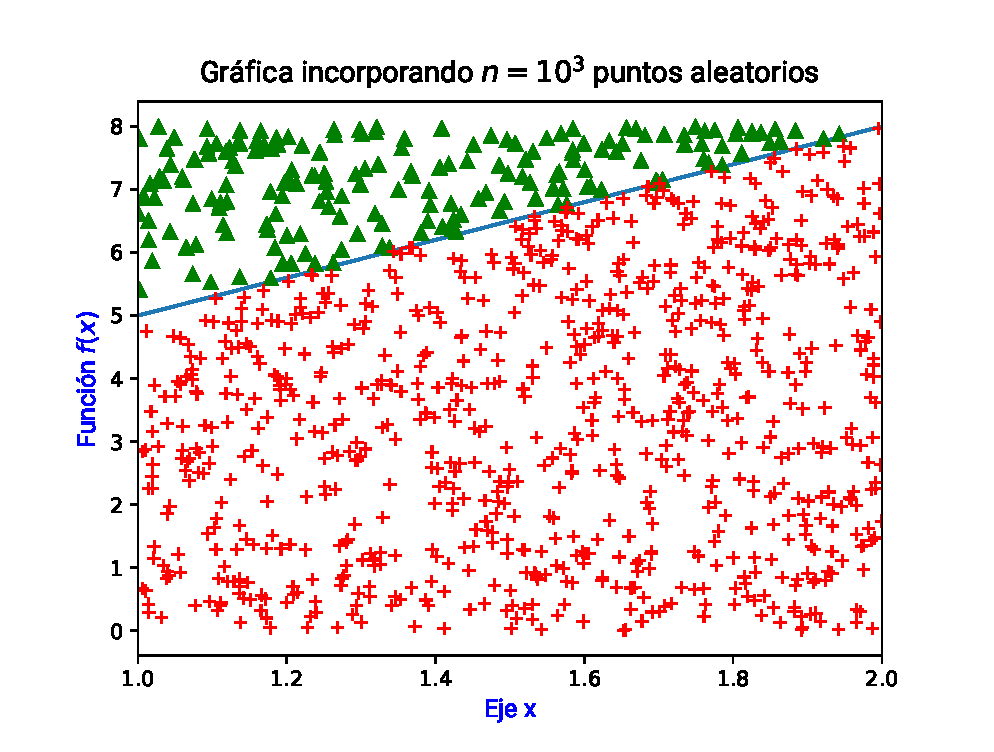
\includegraphics[scale=0.55]{Imagenes/area_puntos_03.eps}
\end{figure}
\end{frame}
\begin{frame}
\frametitle{Gráfica casi completa}
\begin{figure}
    \centering
    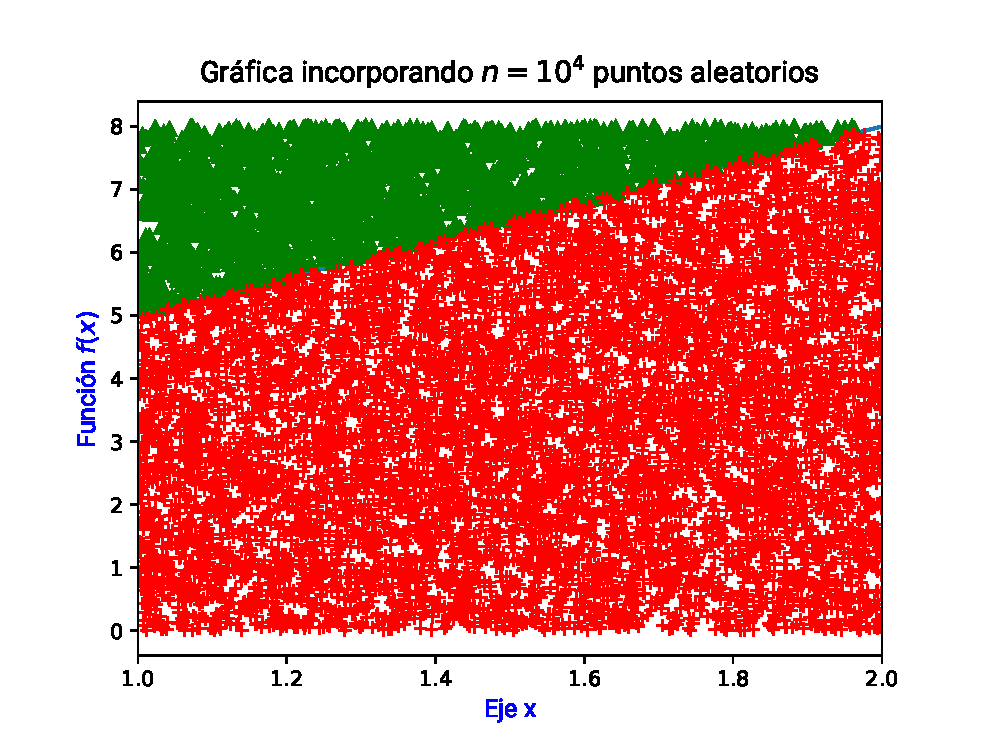
\includegraphics[scale=0.55]{Imagenes/area_puntos_04.eps}
\end{figure}
\end{frame}
\begin{frame}
\frametitle{Gráfica que nos devuelve el valor de la integral}
\begin{figure}
    \centering
    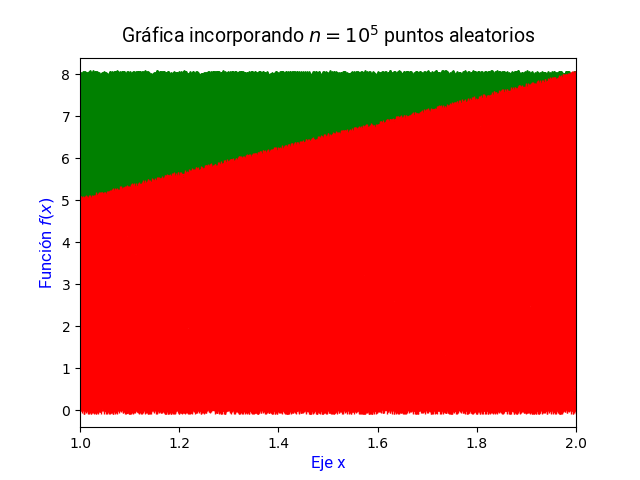
\includegraphics[scale=0.55]{Imagenes/area_puntos_05.png}
\end{figure}
\end{frame}
\begin{frame}
\frametitle{Gráfica con el valor exacto de la integral}
\begin{figure}
    \centering
    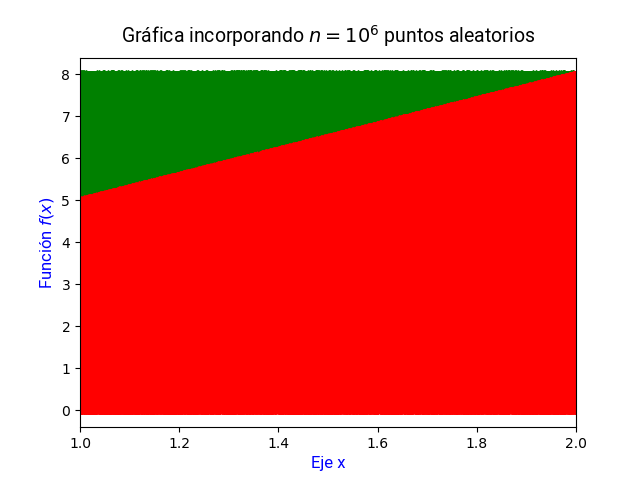
\includegraphics[scale=0.55]{Imagenes/area_puntos_06.png}
\end{figure}
\end{frame}
\begin{frame}
\frametitle{Gráfica del error vs. número de muestras}
\begin{figure}
    \centering
    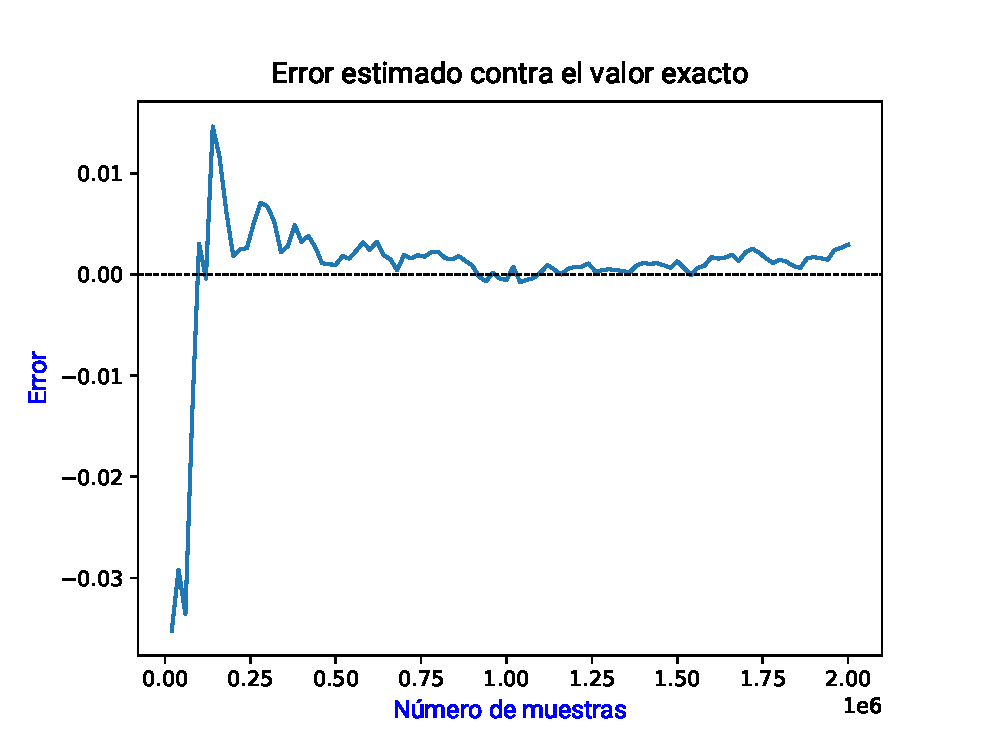
\includegraphics[scale=0.55]{Imagenes/area_puntos_07_error.eps}
\end{figure}
\end{frame}
\end{document}